\documentclass{article}
\usepackage{iclr2027_conference,times}

% Optional notation file distributed with the official ICLR 2027 template.
% Preserve amsmath's parenthesized equation references used by this paper;
% math_commands.tex otherwise redefines \eqref as "equation <number>".
\usepackage{amsmath}
\let\PCeqref\eqref
%%%%% NEW MATH DEFINITIONS %%%%%

\usepackage{amsmath,amsfonts,bm}

% Mark sections of captions for referring to divisions of figures
\newcommand{\figleft}{{\em (Left)}}
\newcommand{\figcenter}{{\em (Center)}}
\newcommand{\figright}{{\em (Right)}}
\newcommand{\figtop}{{\em (Top)}}
\newcommand{\figbottom}{{\em (Bottom)}}
\newcommand{\captiona}{{\em (a)}}
\newcommand{\captionb}{{\em (b)}}
\newcommand{\captionc}{{\em (c)}}
\newcommand{\captiond}{{\em (d)}}

% Highlight a newly defined term
\newcommand{\newterm}[1]{{\bf #1}}


% Figure reference, lower-case.
\def\figref#1{figure~\ref{#1}}
% Figure reference, capital. For start of sentence
\def\Figref#1{Figure~\ref{#1}}
\def\twofigref#1#2{figures \ref{#1} and \ref{#2}}
\def\quadfigref#1#2#3#4{figures \ref{#1}, \ref{#2}, \ref{#3} and \ref{#4}}
% Section reference, lower-case.
\def\secref#1{section~\ref{#1}}
% Section reference, capital.
\def\Secref#1{Section~\ref{#1}}
% Reference to two sections.
\def\twosecrefs#1#2{sections \ref{#1} and \ref{#2}}
% Reference to three sections.
\def\secrefs#1#2#3{sections \ref{#1}, \ref{#2} and \ref{#3}}
% Reference to an equation, lower-case.
\def\eqref#1{equation~\ref{#1}}
% Reference to an equation, upper case
\def\Eqref#1{Equation~\ref{#1}}
% A raw reference to an equation---avoid using if possible
\def\plaineqref#1{\ref{#1}}
% Reference to a chapter, lower-case.
\def\chapref#1{chapter~\ref{#1}}
% Reference to an equation, upper case.
\def\Chapref#1{Chapter~\ref{#1}}
% Reference to a range of chapters
\def\rangechapref#1#2{chapters\ref{#1}--\ref{#2}}
% Reference to an algorithm, lower-case.
\def\algref#1{algorithm~\ref{#1}}
% Reference to an algorithm, upper case.
\def\Algref#1{Algorithm~\ref{#1}}
\def\twoalgref#1#2{algorithms \ref{#1} and \ref{#2}}
\def\Twoalgref#1#2{Algorithms \ref{#1} and \ref{#2}}
% Reference to a part, lower case
\def\partref#1{part~\ref{#1}}
% Reference to a part, upper case
\def\Partref#1{Part~\ref{#1}}
\def\twopartref#1#2{parts \ref{#1} and \ref{#2}}

\def\ceil#1{\lceil #1 \rceil}
\def\floor#1{\lfloor #1 \rfloor}
\def\1{\bm{1}}
\newcommand{\train}{\mathcal{D}}
\newcommand{\valid}{\mathcal{D_{\mathrm{valid}}}}
\newcommand{\test}{\mathcal{D_{\mathrm{test}}}}

\def\eps{{\epsilon}}


% Random variables
\def\reta{{\textnormal{$\eta$}}}
\def\ra{{\textnormal{a}}}
\def\rb{{\textnormal{b}}}
\def\rc{{\textnormal{c}}}
\def\rd{{\textnormal{d}}}
\def\re{{\textnormal{e}}}
\def\rf{{\textnormal{f}}}
\def\rg{{\textnormal{g}}}
\def\rh{{\textnormal{h}}}
\def\ri{{\textnormal{i}}}
\def\rj{{\textnormal{j}}}
\def\rk{{\textnormal{k}}}
\def\rl{{\textnormal{l}}}
% rm is already a command, just don't name any random variables m
\def\rn{{\textnormal{n}}}
\def\ro{{\textnormal{o}}}
\def\rp{{\textnormal{p}}}
\def\rq{{\textnormal{q}}}
\def\rr{{\textnormal{r}}}
\def\rs{{\textnormal{s}}}
\def\rt{{\textnormal{t}}}
\def\ru{{\textnormal{u}}}
\def\rv{{\textnormal{v}}}
\def\rw{{\textnormal{w}}}
\def\rx{{\textnormal{x}}}
\def\ry{{\textnormal{y}}}
\def\rz{{\textnormal{z}}}

% Random vectors
\def\rvepsilon{{\mathbf{\epsilon}}}
\def\rvtheta{{\mathbf{\theta}}}
\def\rva{{\mathbf{a}}}
\def\rvb{{\mathbf{b}}}
\def\rvc{{\mathbf{c}}}
\def\rvd{{\mathbf{d}}}
\def\rve{{\mathbf{e}}}
\def\rvf{{\mathbf{f}}}
\def\rvg{{\mathbf{g}}}
\def\rvh{{\mathbf{h}}}
\def\rvu{{\mathbf{i}}}
\def\rvj{{\mathbf{j}}}
\def\rvk{{\mathbf{k}}}
\def\rvl{{\mathbf{l}}}
\def\rvm{{\mathbf{m}}}
\def\rvn{{\mathbf{n}}}
\def\rvo{{\mathbf{o}}}
\def\rvp{{\mathbf{p}}}
\def\rvq{{\mathbf{q}}}
\def\rvr{{\mathbf{r}}}
\def\rvs{{\mathbf{s}}}
\def\rvt{{\mathbf{t}}}
\def\rvu{{\mathbf{u}}}
\def\rvv{{\mathbf{v}}}
\def\rvw{{\mathbf{w}}}
\def\rvx{{\mathbf{x}}}
\def\rvy{{\mathbf{y}}}
\def\rvz{{\mathbf{z}}}

% Elements of random vectors
\def\erva{{\textnormal{a}}}
\def\ervb{{\textnormal{b}}}
\def\ervc{{\textnormal{c}}}
\def\ervd{{\textnormal{d}}}
\def\erve{{\textnormal{e}}}
\def\ervf{{\textnormal{f}}}
\def\ervg{{\textnormal{g}}}
\def\ervh{{\textnormal{h}}}
\def\ervi{{\textnormal{i}}}
\def\ervj{{\textnormal{j}}}
\def\ervk{{\textnormal{k}}}
\def\ervl{{\textnormal{l}}}
\def\ervm{{\textnormal{m}}}
\def\ervn{{\textnormal{n}}}
\def\ervo{{\textnormal{o}}}
\def\ervp{{\textnormal{p}}}
\def\ervq{{\textnormal{q}}}
\def\ervr{{\textnormal{r}}}
\def\ervs{{\textnormal{s}}}
\def\ervt{{\textnormal{t}}}
\def\ervu{{\textnormal{u}}}
\def\ervv{{\textnormal{v}}}
\def\ervw{{\textnormal{w}}}
\def\ervx{{\textnormal{x}}}
\def\ervy{{\textnormal{y}}}
\def\ervz{{\textnormal{z}}}

% Random matrices
\def\rmA{{\mathbf{A}}}
\def\rmB{{\mathbf{B}}}
\def\rmC{{\mathbf{C}}}
\def\rmD{{\mathbf{D}}}
\def\rmE{{\mathbf{E}}}
\def\rmF{{\mathbf{F}}}
\def\rmG{{\mathbf{G}}}
\def\rmH{{\mathbf{H}}}
\def\rmI{{\mathbf{I}}}
\def\rmJ{{\mathbf{J}}}
\def\rmK{{\mathbf{K}}}
\def\rmL{{\mathbf{L}}}
\def\rmM{{\mathbf{M}}}
\def\rmN{{\mathbf{N}}}
\def\rmO{{\mathbf{O}}}
\def\rmP{{\mathbf{P}}}
\def\rmQ{{\mathbf{Q}}}
\def\rmR{{\mathbf{R}}}
\def\rmS{{\mathbf{S}}}
\def\rmT{{\mathbf{T}}}
\def\rmU{{\mathbf{U}}}
\def\rmV{{\mathbf{V}}}
\def\rmW{{\mathbf{W}}}
\def\rmX{{\mathbf{X}}}
\def\rmY{{\mathbf{Y}}}
\def\rmZ{{\mathbf{Z}}}

% Elements of random matrices
\def\ermA{{\textnormal{A}}}
\def\ermB{{\textnormal{B}}}
\def\ermC{{\textnormal{C}}}
\def\ermD{{\textnormal{D}}}
\def\ermE{{\textnormal{E}}}
\def\ermF{{\textnormal{F}}}
\def\ermG{{\textnormal{G}}}
\def\ermH{{\textnormal{H}}}
\def\ermI{{\textnormal{I}}}
\def\ermJ{{\textnormal{J}}}
\def\ermK{{\textnormal{K}}}
\def\ermL{{\textnormal{L}}}
\def\ermM{{\textnormal{M}}}
\def\ermN{{\textnormal{N}}}
\def\ermO{{\textnormal{O}}}
\def\ermP{{\textnormal{P}}}
\def\ermQ{{\textnormal{Q}}}
\def\ermR{{\textnormal{R}}}
\def\ermS{{\textnormal{S}}}
\def\ermT{{\textnormal{T}}}
\def\ermU{{\textnormal{U}}}
\def\ermV{{\textnormal{V}}}
\def\ermW{{\textnormal{W}}}
\def\ermX{{\textnormal{X}}}
\def\ermY{{\textnormal{Y}}}
\def\ermZ{{\textnormal{Z}}}

% Vectors
\def\vzero{{\bm{0}}}
\def\vone{{\bm{1}}}
\def\vmu{{\bm{\mu}}}
\def\vtheta{{\bm{\theta}}}
\def\va{{\bm{a}}}
\def\vb{{\bm{b}}}
\def\vc{{\bm{c}}}
\def\vd{{\bm{d}}}
\def\ve{{\bm{e}}}
\def\vf{{\bm{f}}}
\def\vg{{\bm{g}}}
\def\vh{{\bm{h}}}
\def\vi{{\bm{i}}}
\def\vj{{\bm{j}}}
\def\vk{{\bm{k}}}
\def\vl{{\bm{l}}}
\def\vm{{\bm{m}}}
\def\vn{{\bm{n}}}
\def\vo{{\bm{o}}}
\def\vp{{\bm{p}}}
\def\vq{{\bm{q}}}
\def\vr{{\bm{r}}}
\def\vs{{\bm{s}}}
\def\vt{{\bm{t}}}
\def\vu{{\bm{u}}}
\def\vv{{\bm{v}}}
\def\vw{{\bm{w}}}
\def\vx{{\bm{x}}}
\def\vy{{\bm{y}}}
\def\vz{{\bm{z}}}

% Elements of vectors
\def\evalpha{{\alpha}}
\def\evbeta{{\beta}}
\def\evepsilon{{\epsilon}}
\def\evlambda{{\lambda}}
\def\evomega{{\omega}}
\def\evmu{{\mu}}
\def\evpsi{{\psi}}
\def\evsigma{{\sigma}}
\def\evtheta{{\theta}}
\def\eva{{a}}
\def\evb{{b}}
\def\evc{{c}}
\def\evd{{d}}
\def\eve{{e}}
\def\evf{{f}}
\def\evg{{g}}
\def\evh{{h}}
\def\evi{{i}}
\def\evj{{j}}
\def\evk{{k}}
\def\evl{{l}}
\def\evm{{m}}
\def\evn{{n}}
\def\evo{{o}}
\def\evp{{p}}
\def\evq{{q}}
\def\evr{{r}}
\def\evs{{s}}
\def\evt{{t}}
\def\evu{{u}}
\def\evv{{v}}
\def\evw{{w}}
\def\evx{{x}}
\def\evy{{y}}
\def\evz{{z}}

% Matrix
\def\mA{{\bm{A}}}
\def\mB{{\bm{B}}}
\def\mC{{\bm{C}}}
\def\mD{{\bm{D}}}
\def\mE{{\bm{E}}}
\def\mF{{\bm{F}}}
\def\mG{{\bm{G}}}
\def\mH{{\bm{H}}}
\def\mI{{\bm{I}}}
\def\mJ{{\bm{J}}}
\def\mK{{\bm{K}}}
\def\mL{{\bm{L}}}
\def\mM{{\bm{M}}}
\def\mN{{\bm{N}}}
\def\mO{{\bm{O}}}
\def\mP{{\bm{P}}}
\def\mQ{{\bm{Q}}}
\def\mR{{\bm{R}}}
\def\mS{{\bm{S}}}
\def\mT{{\bm{T}}}
\def\mU{{\bm{U}}}
\def\mV{{\bm{V}}}
\def\mW{{\bm{W}}}
\def\mX{{\bm{X}}}
\def\mY{{\bm{Y}}}
\def\mZ{{\bm{Z}}}
\def\mBeta{{\bm{\beta}}}
\def\mPhi{{\bm{\Phi}}}
\def\mLambda{{\bm{\Lambda}}}
\def\mSigma{{\bm{\Sigma}}}

% Tensor
\DeclareMathAlphabet{\mathsfit}{\encodingdefault}{\sfdefault}{m}{sl}
\SetMathAlphabet{\mathsfit}{bold}{\encodingdefault}{\sfdefault}{bx}{n}
\newcommand{\tens}[1]{\bm{\mathsfit{#1}}}
\def\tA{{\tens{A}}}
\def\tB{{\tens{B}}}
\def\tC{{\tens{C}}}
\def\tD{{\tens{D}}}
\def\tE{{\tens{E}}}
\def\tF{{\tens{F}}}
\def\tG{{\tens{G}}}
\def\tH{{\tens{H}}}
\def\tI{{\tens{I}}}
\def\tJ{{\tens{J}}}
\def\tK{{\tens{K}}}
\def\tL{{\tens{L}}}
\def\tM{{\tens{M}}}
\def\tN{{\tens{N}}}
\def\tO{{\tens{O}}}
\def\tP{{\tens{P}}}
\def\tQ{{\tens{Q}}}
\def\tR{{\tens{R}}}
\def\tS{{\tens{S}}}
\def\tT{{\tens{T}}}
\def\tU{{\tens{U}}}
\def\tV{{\tens{V}}}
\def\tW{{\tens{W}}}
\def\tX{{\tens{X}}}
\def\tY{{\tens{Y}}}
\def\tZ{{\tens{Z}}}


% Graph
\def\gA{{\mathcal{A}}}
\def\gB{{\mathcal{B}}}
\def\gC{{\mathcal{C}}}
\def\gD{{\mathcal{D}}}
\def\gE{{\mathcal{E}}}
\def\gF{{\mathcal{F}}}
\def\gG{{\mathcal{G}}}
\def\gH{{\mathcal{H}}}
\def\gI{{\mathcal{I}}}
\def\gJ{{\mathcal{J}}}
\def\gK{{\mathcal{K}}}
\def\gL{{\mathcal{L}}}
\def\gM{{\mathcal{M}}}
\def\gN{{\mathcal{N}}}
\def\gO{{\mathcal{O}}}
\def\gP{{\mathcal{P}}}
\def\gQ{{\mathcal{Q}}}
\def\gR{{\mathcal{R}}}
\def\gS{{\mathcal{S}}}
\def\gT{{\mathcal{T}}}
\def\gU{{\mathcal{U}}}
\def\gV{{\mathcal{V}}}
\def\gW{{\mathcal{W}}}
\def\gX{{\mathcal{X}}}
\def\gY{{\mathcal{Y}}}
\def\gZ{{\mathcal{Z}}}

% Sets
\def\sA{{\mathbb{A}}}
\def\sB{{\mathbb{B}}}
\def\sC{{\mathbb{C}}}
\def\sD{{\mathbb{D}}}
% Don't use a set called E, because this would be the same as our symbol
% for expectation.
\def\sF{{\mathbb{F}}}
\def\sG{{\mathbb{G}}}
\def\sH{{\mathbb{H}}}
\def\sI{{\mathbb{I}}}
\def\sJ{{\mathbb{J}}}
\def\sK{{\mathbb{K}}}
\def\sL{{\mathbb{L}}}
\def\sM{{\mathbb{M}}}
\def\sN{{\mathbb{N}}}
\def\sO{{\mathbb{O}}}
\def\sP{{\mathbb{P}}}
\def\sQ{{\mathbb{Q}}}
\def\sR{{\mathbb{R}}}
\def\sS{{\mathbb{S}}}
\def\sT{{\mathbb{T}}}
\def\sU{{\mathbb{U}}}
\def\sV{{\mathbb{V}}}
\def\sW{{\mathbb{W}}}
\def\sX{{\mathbb{X}}}
\def\sY{{\mathbb{Y}}}
\def\sZ{{\mathbb{Z}}}

% Entries of a matrix
\def\emLambda{{\Lambda}}
\def\emA{{A}}
\def\emB{{B}}
\def\emC{{C}}
\def\emD{{D}}
\def\emE{{E}}
\def\emF{{F}}
\def\emG{{G}}
\def\emH{{H}}
\def\emI{{I}}
\def\emJ{{J}}
\def\emK{{K}}
\def\emL{{L}}
\def\emM{{M}}
\def\emN{{N}}
\def\emO{{O}}
\def\emP{{P}}
\def\emQ{{Q}}
\def\emR{{R}}
\def\emS{{S}}
\def\emT{{T}}
\def\emU{{U}}
\def\emV{{V}}
\def\emW{{W}}
\def\emX{{X}}
\def\emY{{Y}}
\def\emZ{{Z}}
\def\emSigma{{\Sigma}}

% entries of a tensor
% Same font as tensor, without \bm wrapper
\newcommand{\etens}[1]{\mathsfit{#1}}
\def\etLambda{{\etens{\Lambda}}}
\def\etA{{\etens{A}}}
\def\etB{{\etens{B}}}
\def\etC{{\etens{C}}}
\def\etD{{\etens{D}}}
\def\etE{{\etens{E}}}
\def\etF{{\etens{F}}}
\def\etG{{\etens{G}}}
\def\etH{{\etens{H}}}
\def\etI{{\etens{I}}}
\def\etJ{{\etens{J}}}
\def\etK{{\etens{K}}}
\def\etL{{\etens{L}}}
\def\etM{{\etens{M}}}
\def\etN{{\etens{N}}}
\def\etO{{\etens{O}}}
\def\etP{{\etens{P}}}
\def\etQ{{\etens{Q}}}
\def\etR{{\etens{R}}}
\def\etS{{\etens{S}}}
\def\etT{{\etens{T}}}
\def\etU{{\etens{U}}}
\def\etV{{\etens{V}}}
\def\etW{{\etens{W}}}
\def\etX{{\etens{X}}}
\def\etY{{\etens{Y}}}
\def\etZ{{\etens{Z}}}

% The true underlying data generating distribution
\newcommand{\pdata}{p_{\rm{data}}}
% The empirical distribution defined by the training set
\newcommand{\ptrain}{\hat{p}_{\rm{data}}}
\newcommand{\Ptrain}{\hat{P}_{\rm{data}}}
% The model distribution
\newcommand{\pmodel}{p_{\rm{model}}}
\newcommand{\Pmodel}{P_{\rm{model}}}
\newcommand{\ptildemodel}{\tilde{p}_{\rm{model}}}
% Stochastic autoencoder distributions
\newcommand{\pencode}{p_{\rm{encoder}}}
\newcommand{\pdecode}{p_{\rm{decoder}}}
\newcommand{\precons}{p_{\rm{reconstruct}}}

\newcommand{\laplace}{\mathrm{Laplace}} % Laplace distribution

\newcommand{\E}{\mathbb{E}}
\newcommand{\Ls}{\mathcal{L}}
\newcommand{\R}{\mathbb{R}}
\newcommand{\emp}{\tilde{p}}
\newcommand{\lr}{\alpha}
\newcommand{\reg}{\lambda}
\newcommand{\rect}{\mathrm{rectifier}}
\newcommand{\softmax}{\mathrm{softmax}}
\newcommand{\sigmoid}{\sigma}
\newcommand{\softplus}{\zeta}
\newcommand{\KL}{D_{\mathrm{KL}}}
\newcommand{\Var}{\mathrm{Var}}
\newcommand{\standarderror}{\mathrm{SE}}
\newcommand{\Cov}{\mathrm{Cov}}
% Wolfram Mathworld says $L^2$ is for function spaces and $\ell^2$ is for vectors
% But then they seem to use $L^2$ for vectors throughout the site, and so does
% wikipedia.
\newcommand{\normlzero}{L^0}
\newcommand{\normlone}{L^1}
\newcommand{\normltwo}{L^2}
\newcommand{\normlp}{L^p}
\newcommand{\normmax}{L^\infty}

\newcommand{\parents}{Pa} % See usage in notation.tex. Chosen to match Daphne's book.

\DeclareMathOperator*{\argmax}{arg\,max}
\DeclareMathOperator*{\argmin}{arg\,min}

\DeclareMathOperator{\sign}{sign}
\DeclareMathOperator{\Tr}{Tr}
\let\ab\allowbreak

\let\eqref\PCeqref

% Paper-specific packages; the official style controls the page layout.
\usepackage[T1]{fontenc}
\usepackage[utf8]{inputenc}
\usepackage{amssymb,amsthm,booktabs,tabularx,graphicx}
\usepackage{microtype,xcolor}
\usepackage{enumitem}
\usepackage{hyperref}
\usepackage{url}
\hypersetup{hidelinks}

% Paper-specific environments and macros (\E comes from math_commands.tex).
\newtheorem{theorem}{Theorem}
\newtheorem{proposition}[theorem]{Proposition}
\newtheorem{corollary}[theorem]{Corollary}
\newcommand{\Prb}{\mathbb{P}}
\newcommand{\ind}{\mathbf{1}}
\newcommand{\TV}{\operatorname{TV}}
\newcommand{\TBD}{\textcolor{gray}{TBD}}
\makeatletter
\let\inputrows\@@input
\makeatother
\title{Path-consistency with Prefix Enhancement for Efficient Inference in LLMs}
\author{Anonymous authors}
% Working draft. Do not enable final-copy mode before author review.
%\iclrfinalcopy % Uncomment only for the camera-ready version.
\begin{document}
\maketitle
\begin{abstract}
Self-consistency improves reasoning by aggregating multiple sampled solutions, but generating each trajectory from scratch incurs substantial inference cost. Path-consistency reduces this cost by sharing a continuous reasoning prefix across successive sampling windows. Answer agreement guides prefix extension, while subsequent windows determine whether to commit the proposed prefix or roll back to an earlier one. All valid answers from completed windows contribute to the final vote. We derive an exact finite-horizon decomposition of the gains and losses in voting accuracy induced by prefix reuse. We also establish a voting error bound for adaptive sampling with finitely many competing answers under explicit conditional-margin assumptions. Our evaluation targets three models of different scales, Llama-3.1-8B-Instruct, Qwen3-30B-A3B, and DeepSeek-V4-Flash, across five reasoning benchmarks. Across the five completed comparisons reported in the main text, path-consistency reduces generated tokens by 25.8\% to 39.4\%, averaging 30.8\% across settings, while largely maintaining accuracy under the reported grading procedures. Combining path-consistency with early-stopping methods yields a further 7\% reduction. These results position path-consistency as a competitive reasoning-sharing method that also integrates flexibly with early-stopping methods for additional savings.
\end{abstract}

\section{Introduction}
% Citation needed for self-consistency and its sampling-and-voting procedure.
Self-consistency samples several reasoning trajectories and aggregates their answers.
Its cost grows with the amount of generated reasoning. Even when early samples have found a useful intermediate calculation, later trajectories ordinarily start again from the original question. This suggests reusing part of an earlier solution while continuing to sample diverse suffixes. The potential saving comes from generating less new text per trajectory. Figure~\ref{fig:overview} illustrates the observed repetition and contrasts independent sampling with shared-prefix reuse.

\begin{figure}[t]
\centering
% Author-supplied PDFs are included unchanged and retain vector graphics.
% Bottom alignment places the (b) and (c) caption baselines at the same height.
\begin{minipage}[b]{0.435\linewidth}
\centering
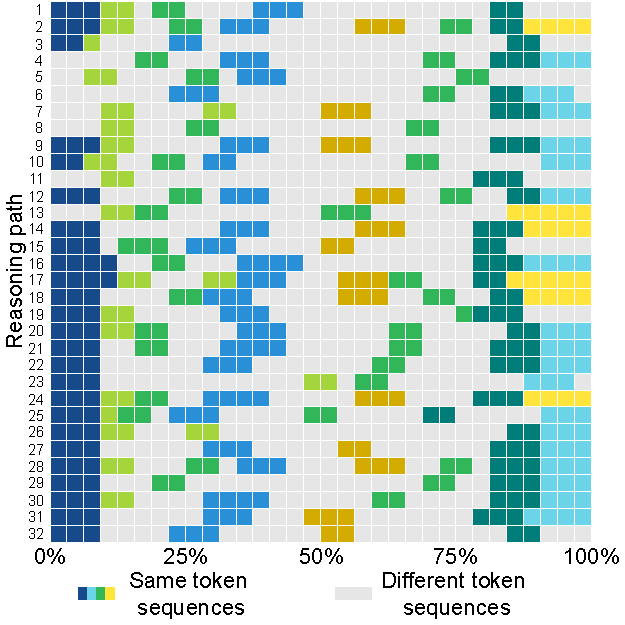
\includegraphics[width=\linewidth]{figs/SC_matrix.pdf}
\par\smallskip
{\small\textbf{(a) SC: independently sampled paths}}
\par\medskip
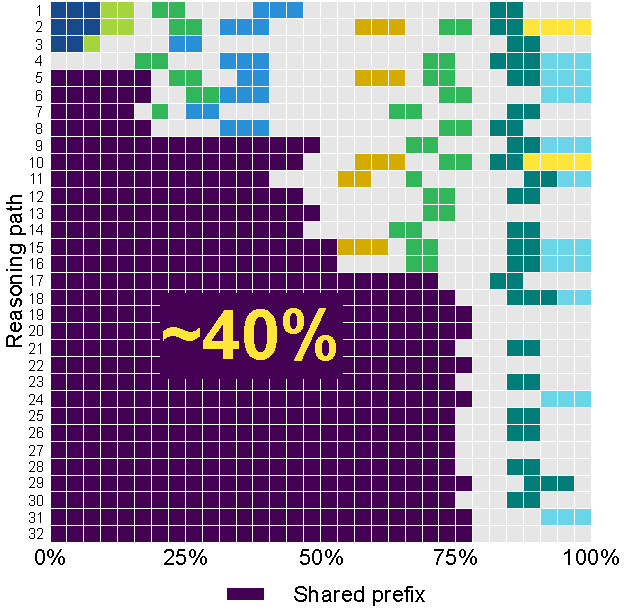
\includegraphics[width=\linewidth]{figs/PC_matrix.pdf}
\par\smallskip
{\small\textbf{(b) PC: shared-prefix reuse}}
\end{minipage}\hfill
\begin{minipage}[b]{0.545\linewidth}
\centering
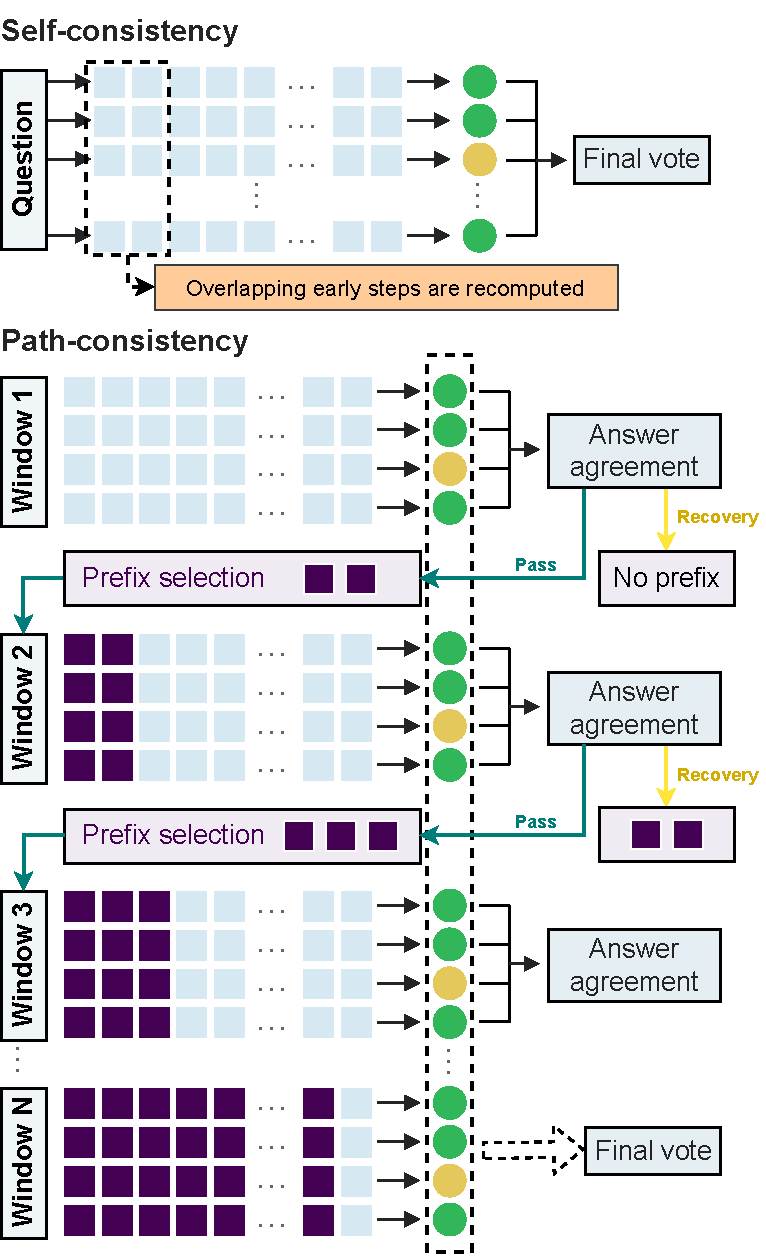
\includegraphics[width=\linewidth]{figs/overview.pdf}
\par\smallskip
{\small\textbf{(c) Overview of SC and PC}}
\end{minipage}

% Citations may be added for GSM8K and Llama-3.1 at their first formal introduction.
% The repetition visualization and token-saving result are evidence from our experiments.
\caption{From repeated reasoning to shared-prefix reuse. (a,b) SC and PC on the same GSM8K question using Llama-3.1-8B-Instruct. Each matrix shows 32 reasoning paths over 32 relative token intervals. Matching colors mark repeated token sequences, purple marks shared prefixes, and gray marks other content. The $\sim$40\% denotes average token savings on GSM8K. (c) SC samples independent paths, whereas PC progressively reuses prefixes across windows. Circles represent answers, with colors indicating answer categories.}
\label{fig:overview}
\end{figure}

We propose path-consistency, a method for token-efficient reasoning through controlled prefix reuse across sampling windows. After a window finishes, answer agreement determines whether to propose a prefix extension. Path-consistency selects a continuous prefix from a trajectory supporting the modal answer and uses it to condition the next window. Subsequent windows test whether to commit the proposal or recover an earlier prefix. Later trajectories therefore reuse part of the reasoning already generated and sample new continuations, while all valid answers contribute to the final vote.

Path-consistency has three practical advantages. First, it reduces the amount of new reasoning generated per trajectory while retaining multiple sampled continuations and answer aggregation. Second, it requires no training, fine-tuning, or architectural changes, operating entirely at inference time through answer agreement, prefix selection, and trial and recovery. Third, prefix reuse is compatible with different autoregressive language models and can be combined with early-stopping methods for additional token savings. These properties make path-consistency a flexible component for efficient multi-path reasoning.

% Citations may be added for the evaluated models and benchmarks at their formal introduction.
% Citations needed for reasoning-sharing and early-stopping baselines at their formal introduction.
% The evaluation overview uses the intended complete-paper framing. Verify Qwen coverage against the final tables before submission.
% The numerical range and mean below refer only to Llama/GSM8K and the four DeepSeek main-table comparisons, not to pending Qwen results.
We evaluate path-consistency using three models of different scales, Llama-3.1-8B-Instruct, DeepSeek-V4-Flash, and Qwen3-30B-A3B, across five reasoning benchmarks. We first examine how shared prefixes progressively extend across sampling windows on Llama-3.1 and GSM8K, then present the main results on DeepSeek and Qwen. On Llama/GSM8K and the four DeepSeek main-table benchmarks, path-consistency reduces generated tokens by 25.8\% to 39.4\%, averaging 30.8\% across these settings, while largely maintaining accuracy. Comparisons with reasoning-sharing methods assess path-consistency's accuracy and token efficiency, and combinations with early-stopping methods demonstrate additional savings. Finally, ablation studies examine the roles of source selection and recovery, as well as how the answer agreement threshold governs prefix reuse and informs operating-point selection.

\section{Background and Related Work}
% Citation needed for self-consistency and answer aggregation.
Self-consistency samples multiple reasoning trajectories and aggregates their answers by voting. Its generation cost can be reduced through early stopping or by sharing previously generated reasoning.

\paragraph{Early-stopping methods.}
These methods decide when to stop sampling or generation.
% Citations needed for AC and ESC and their respective stopping criteria.
Adaptive-Consistency (AC) uses cumulative answer agreement, whereas Early-Stopping Self-Consistency (ESC) uses agreement within a sampling window to stop further sampling.
% Citation needed for DeepConf, distinguishing its online and offline variants.
DeepConf uses model-internal confidence to filter traces during or after generation, although only online termination avoids generating further tokens. Path-consistency instead controls the starting prefix of later trajectories and can complement early-stopping methods while retaining their stopping and aggregation rules.

\paragraph{Reasoning-sharing methods.}
These methods reuse information from sampled trajectories to guide subsequent reasoning.
% Citation needed for Progressive-Hint Prompting and its combination with SC.
Progressive-Hint Prompting reuses previous answers as hints.
% Citation needed for PoLR and its prefix-clustering procedure.
PoLR clusters short prefixes and expands trajectories in the dominant cluster.
% Citation needed for CPT and its pooled intermediate-information sharing.
CPT pools and deduplicates intermediate information for sharing across branches. Path-consistency belongs to this family but shares one continuous reasoning prefix $z$ within each sampling window. Answer agreement gates its extension, prefix selection chooses its source, and trial and recovery determine whether to retain or retract it.

\section{Path-consistency}
\label{sec:method}
Path-consistency reduces repeated reasoning by reusing a continuous prefix across sampling windows and testing its extensions with subsequent samples. Its three components are answer agreement, prefix selection, and trial and recovery, as illustrated in Figure~\ref{fig:loop} and described below. Figure~\ref{fig:overview} shows the overall workflow. The default main setting uses a trajectory budget $B=32$, window size $m=4$, and prefix levels $\mathcal R=\{0,0.2,0.4,0.6,0.8\}$. A prefix level $r\in\mathcal R$ specifies the nominal fraction of the source trajectory's reasoning tokens retained as the shared prefix, excluding the final answer. For example, $r=0.2$ retains approximately the first 20\% of that reasoning, while $r=0$ means no prefix reuse. All trajectories within a window use the same prefix. Path-consistency updates its prefix and agreement statistics only after all trajectories in that window have finished. Self-consistency and path-consistency use the same maximum budget and final majority-vote rule.

\begin{figure}[t]
\centering
% Author-redrawn vector panels supplied in figs/.
% Equal image heights preserve aspect ratios and align all caption baselines.
\begingroup
\edef\PCMethodPanelHeight{\the\dimexpr0.403\linewidth\relax}
\begin{minipage}[t]{0.31\linewidth}
\vspace{0pt}\centering
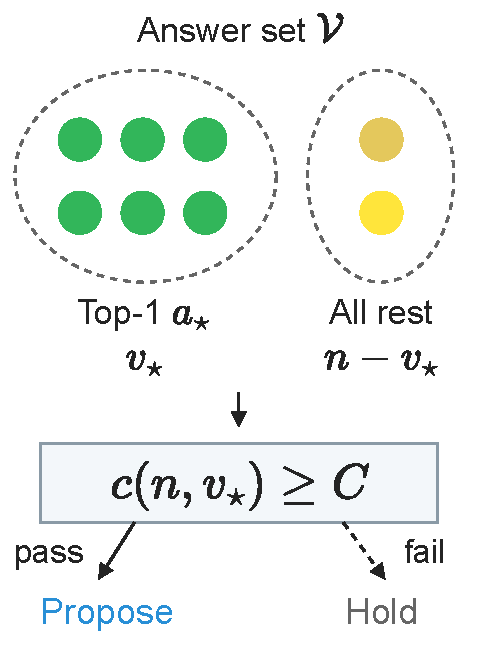
\includegraphics[height=\PCMethodPanelHeight]{figs/method_1.pdf}
\par\smallskip
{\small\textbf{(a) Answer agreement}}
\end{minipage}\hfill
\begin{minipage}[t]{0.326\linewidth}
\vspace{0pt}\centering
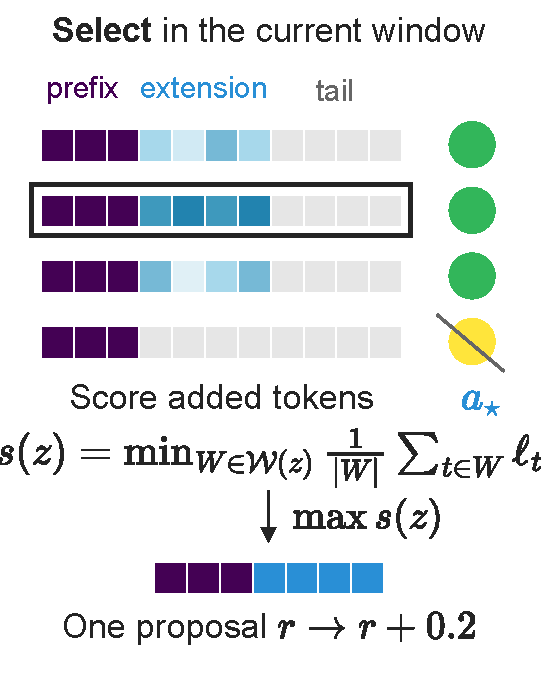
\includegraphics[height=\PCMethodPanelHeight]{figs/method_2.pdf}
\par\smallskip
{\small\textbf{(b) Prefix selection}}
\end{minipage}\hfill
\begin{minipage}[t]{0.332\linewidth}
\vspace{0pt}\centering
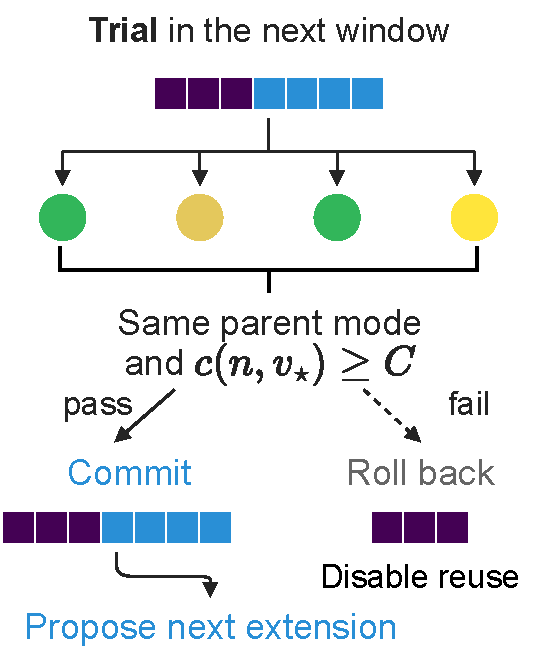
\includegraphics[height=\PCMethodPanelHeight]{figs/method_3.pdf}
\par\smallskip
{\small\textbf{(c) Trial and recovery}}
\end{minipage}
\endgroup

\caption{The three components of PC. (a) Answer agreement determines whether to propose a prefix extension. (b) Local confidence selection chooses an extension from eligible trajectories. (c) Trial and recovery validate the proposal, enabling further extension on success or returning to an earlier prefix on failure. Purple denotes inherited prefixes and blue denotes new extensions. Circles represent answers, with colors indicating answer categories.}
\label{fig:loop}
\end{figure}

\subsection{Answer agreement gate}
Let $\mathcal V$ contain the valid answers admitted by previous successful windows, let $n=|\mathcal V|$, and let $v_\star$ be the count of its modal answer $a_\star$. We use the top-1-versus-all-rest score
\begin{equation}
 c(n,v_\star)=1-I_{1/2}(v_\star+1,n-v_\star+1),
 \label{eq:beta}
\end{equation}
where $I_x$ is the regularized incomplete beta function. For a \emph{fixed} answer category with independent Bernoulli observations and a uniform prior, this is the posterior probability that its mass exceeds $1/2$. In path-consistency the category is selected from the data, successive windows use different prefixes, and unsuccessful windows are excluded from $\mathcal V$. Thus Equation~\ref{eq:beta} is an operational agreement score, not a calibrated posterior over correctness or an anytime error bound.

A nonempty answer set with $c\geq C$ permits a proposal. We fix $C=0.8$ in the main experiments as the default operating point, without selecting it on a development or test set. Threshold sweeps are sensitivity analyses only. At $C=1$ no finite-sample Beta score reaches the threshold in exact arithmetic, recovering self-consistency. A setting of $C=0$ removes the confidence barrier but still requires a valid modal answer and a feasible prefix.

\subsection{Selecting a single continuous prefix}
Once answer agreement permits an extension, path-consistency selects a source trajectory from the just-completed, accepted window. Eligible trajectories must support the modal answer $a_\star$. For a current prefix level $r<0.8$, each trajectory proposes a candidate prefix $z$ ending at $\lfloor(r+0.2)L\rfloor$, where $L$ counts all reasoning tokens in that trajectory, including the inherited prefix but excluding the final answer. Thus each proposal targets the next 20\% level while preserving the existing prefix. The endpoint may be moved backward by up to 32 tokens to avoid explicit answer markers and unbalanced braces or code fences, with punctuation boundaries preferred. Only candidates that extend the current prefix are retained.

We use local confidence selection to rank these candidates using only their newly added tokens. Let $\ell_t$ be the log probability assigned to token $t$ when it was sampled, and let $\mathcal W(z)$ contain the sliding token windows over the added segment of candidate $z$. We define
\begin{equation}
 s(z)=\min_{W\in\mathcal W(z)}\frac{1}{|W|}\sum_{t\in W}\ell_t,
 \label{eq:blc}
\end{equation}
where $W$ is a token window and $|W|$ is its number of scored tokens. The score is the lowest mean log probability across these windows, so choosing the largest $s(z)$ favors candidates whose least confident segment has the highest score. Scoring excludes the inherited prefix, which is shared by all candidates. We use windows of 128 tokens with stride 64 and include the final window; segments shorter than 128 tokens are scored as a whole.

Ties are resolved by fewer generated source tokens and then branch ID. Missing or nonfinite log probabilities are omitted. A candidate with no usable scores receives $-\infty$, and if all candidates receive this value, the same tie-breaking rule selects the source.

\subsection{Trial, commitment, and rollback}
As illustrated in Figure~\ref{fig:loop}(c), a proposed prefix is used for the next sampling window as a trial. After that window finishes, we compute the agreement score in Equation~\ref{eq:beta} using $\mathcal V$ together with the trial's valid answers. The trial succeeds if the modal answer remains the same as when the prefix was proposed and the score is at least $C$. We then commit the prefix, add the trial's valid answers to $\mathcal V$, and reset the consecutive-failure counter.

The same agreement score also gates the next prefix extension. Since a successful trial has already met the threshold, no additional agreement calculation is needed after commitment. If sampling budget remains and the prefix level is below 0.8, the accepted window supplies candidate extensions at the next level using the selection procedure above. A feasible selected extension becomes the next trial; otherwise, sampling continues with the committed prefix. Thus one window can both validate the preceding proposal and supply the next extension.

If a trial fails, we discard its proposed prefix and return to the last committed prefix. A failed monitoring window at an already committed prefix rolls back one level. Two consecutive failures clear the prefix stack and disable further prefix reuse for that question. Failed-window answers are excluded from subsequent agreement calculations and source selection, but all valid answers still contribute to the final vote and the full generation cost is counted. Earlier admitted answers remain in $\mathcal V$ after rollback.

At root, valid answers enter $\mathcal V$ even if confidence is too low to propose a prefix. The algorithm stays at the current level when there is no feasible extension, and cannot extend past the nominal 80\% level. Because each new source can have a different length, a level is a fraction of that source, not a fixed absolute number of tokens. Appendix~\ref{app:algorithm} gives the state transitions used in the runs.

\section{Voting Accuracy under Prefix Reuse}
\label{sec:theory}
Prefix reuse reduces repeated generation but also changes the answer distributions and the dependence between sampled trajectories. We study how these changes affect final voting accuracy relative to self-consistency, and under what conditions voting remains reliable with adaptive sampling. First, we derive an exact decomposition of the accuracy difference into the expected contributions of individual windows. Second, we bound voting error when the correct answer has a sufficient accumulated conditional advantage over every competing answer. Together, these results characterize the benefits and risks of prefix reuse without assuming that answer agreement implies correctness. All probabilities concern a fixed question with correct answer $a^\star$, and multiple incorrect answers are allowed. The analysis uses standard telescoping and bounded-martingale arguments, with proofs in Appendix~\ref{app:proofs}.

\subsection{Decomposing the effect of prefix reuse on accuracy}
Let $H_j$ be the complete history before window $j\in\{0,\ldots,J-1\}$, including traces and controller state. A kernel $K_j^{P}(\cdot\mid h)$ generates the next window under path-consistency. Define $K_j^{S}(\cdot\mid h)$ to generate an unprefixed self-consistency window from any history $h$, including histories created by path-consistency. Let $V_j^S(h)\in[0,1]$ be the probability of final voting correctness if all remaining windows use these self-consistency kernels. The terminal value $V_J^S$ is the correctness indicator under a fixed tie rule. This construction retains all earlier votes when switching to self-consistency.

\begin{theorem}[Exact intervention decomposition]
\label{thm:decomposition}
For a fixed finite budget and common initial state, define
\begin{equation}
 d_j(h)=\int V_{j+1}^{S}(h,u)\,
       [K_j^{P}(du\mid h)-K_j^{S}(du\mid h)].
\end{equation}
Then the difference in final accuracy is exactly
\begin{equation}
 A_P-A_S=\sum_{j=0}^{J-1}\E_{H_j\sim P}[d_j(H_j)].
 \label{eq:risk}
\end{equation}
In particular, if every expected increment is nonnegative, $A_P\geq A_S$. In general,
\begin{equation}
 |A_P-A_S|\leq
 \min\left\{1,\sum_{j=0}^{J-1}\E_P\TV(K_j^P(\cdot\mid H_j),K_j^S(\cdot\mid H_j))\right\}.
 \label{eq:tv}
\end{equation}
\end{theorem}

Writing $d_j^+=\max(d_j,0)$ and $d_j^-=\max(-d_j,0)$ separates the accuracy change into total expected benefit minus total expected harm. This identity includes selection, correlation, failed trials, and rollback through the history and kernels. It makes no small-perturbation approximation. The sufficient condition is deliberately explicit: agreement does not establish the sign of $d_j$, since $V^S$ depends on correctness and remaining votes. A root window has identical conditional kernels and zero increment, even after earlier prefixes changed its history. Rollback can eliminate further prefix-induced increments but cannot undo earlier votes.

\subsection{Bounding voting error under adaptive sampling}
Consider a fixed finite answer alphabet $\mathcal A$ containing $a^\star$. Invalid outputs may be included as a separate symbol. Expose the $B$ sampled answers sequentially, using a filtration $\mathcal F_i$ that includes the information controlling their generation. For competitor $a\neq a^\star$, set
\[
 X_i(a)=\ind\{A_i=a^\star\}-\ind\{A_i=a\},\qquad
 \mu_i(a)=\E[X_i(a)\mid\mathcal F_{i-1}].
\]
\begin{theorem}[Plurality under conditional margins]
\label{thm:plurality}
If deterministic constants $\Gamma_a>0$ satisfy
$\sum_{i=1}^B\mu_i(a)\geq\Gamma_a$ almost surely for every incorrect answer, then
\begin{equation}
 \Prb(\widehat A\neq a^\star)
 \leq \min\left\{1,\sum_{a\neq a^\star}
                  \exp\left(-\frac{\Gamma_a^2}{2B}\right)\right\}.
 \label{eq:margin}
\end{equation}
Ties are treated as failures, so the bound also covers any deterministic tie rule. If invalid answers are discarded, bounding a loss to the invalid symbol is conservative.
\end{theorem}

The bound accommodates adaptive, non-identically distributed samples and requires an accumulated conditional advantage over each incorrect answer, rather than a correct-answer probability above $1/2$. It therefore allows errors to be distributed among multiple answers. This condition is not established by observed marginal accuracy or a high Beta score, and an early incorrect prefix can reverse subsequent conditional advantages. The bound is informative only for sufficiently large margins and may be vacuous at $B=32$. Applying it to open-ended answers also requires justification of the finite-support assumption.

Together, the two results distinguish accuracy preservation from voting reliability. Theorem~\ref{thm:decomposition} shows that prefix reuse preserves accuracy relative to self-consistency when its total expected benefit offsets its total expected harm. Theorem~\ref{thm:plurality} bounds the absolute voting error under sufficient conditional advantages, even when sampling adapts to earlier outcomes. These results provide a framework for analyzing path-consistency, not an unconditional guarantee for its agreement gate. Whether prefix selection and recovery achieve a favorable accuracy--cost trade-off is assessed empirically in Section~\ref{sec:evaluation}.

\section{Evaluation}
\label{sec:evaluation}
\subsection{Experimental setup}
\label{sec:setup}
\paragraph{Models.}
% Citations needed for Llama-3.1, DeepSeek-V4-Flash, Qwen3, and vLLM.
We use Llama-3.1-8B-Instruct, DeepSeek-V4-Flash, and Qwen3-30B-A3B. Llama supports the analysis of prefix reuse and the comparison and composition experiments on GSM8K, while DeepSeek and Qwen are used for the main benchmark comparisons. DeepSeek and Qwen operate with thinking enabled. Llama uses its chat template and is served through vLLM on RTX 4090 hardware; DeepSeek is accessed through its API.

\paragraph{Datasets.}
% Citations needed for GSM8K, MATH-500, AIME 2024/2025, and GPQA-Diamond.
We evaluate on five reasoning benchmarks. GSM8K contains 1,319 test questions, MATH-500 reports accuracy over 500 questions (490 evaluated, with the ten held out for engineering debugging counted as correct), AIME 2024 and AIME 2025 each contain 30 questions, and GPQA-Diamond contains 198 questions. Dataset sources, exclusions, and grading procedures are provided in Appendix~\ref{app:protocol}. Token means on MATH-500 use the 490 generated questions. We report voting accuracy and mean generated tokens per question. Pass@1 denotes the accuracy of the first trajectory in the self-consistency pool rather than greedy decoding.

\paragraph{Hyperparameters.}
Self-consistency and path-consistency use a trajectory budget of $B=32$ and a sampling window of $m=4$. Path-consistency uses the default agreement threshold $C=0.8$ and the fixed prefix levels $\mathcal R=\{0,0.2,0.4,0.6,0.8\}$. For Llama/GSM8K, we use temperature 0.6, top-$p=0.9$, no top-$k$ filtering, and a 2,048-token generation limit. Qwen uses temperature 0.6, top-$p=0.95$, top-$k=20$, and a 32,768-token limit. DeepSeek uses high reasoning effort and a 32,768-token limit. Token costs count newly generated reasoning and answer tokens, including failed windows and the original cost of reused self-consistency roots. Generation time is compared only within the same model and dataset and uses the same inclusive accounting, as detailed in Appendix~\ref{app:protocol}.

\subsection{Progressive prefix reuse and token savings}
\label{sec:llama}
\label{sec:windows}
We use Llama-3.1-8B-Instruct on GSM8K to examine how path-consistency progressively extends a shared prefix and reduces the cost of later sampling windows. Path-consistency reduces mean generated tokens from 8,316 to 5,039 and inclusive generation time from 54.4 to 33.8 seconds per question, with final accuracy of 91.74\% versus 92.12\% for self-consistency.

\begin{figure}[t]
\centering
\begin{minipage}[c]{0.69\linewidth}
\centering
\setlength{\abovecaptionskip}{3pt}
\setlength{\belowcaptionskip}{3pt}
\makeatletter\def\@captype{table}\makeatother
\caption{Prefix reuse on Llama/GSM8K.}
\label{tab:prefix_levels}
\begingroup
\small
\setlength{\tabcolsep}{4pt}
\renewcommand{\arraystretch}{1.25}
\begin{tabular*}{\linewidth}{@{\extracolsep{\fill}}lrrrrr@{}}
\toprule
Level & Windows & Prefix & Tokens & Save (\%) & Time (\%)\\
\midrule
\inputrows{tables/prefix_level_rows.tex}
\bottomrule
\end{tabular*}
\endgroup
\end{minipage}\hspace{0.025\linewidth}%
% Narrow the figure block without scaling the caption typography.
\begin{minipage}[c]{0.28\linewidth}
\centering
\setlength{\abovecaptionskip}{3pt}
\setlength{\belowcaptionskip}{0pt}
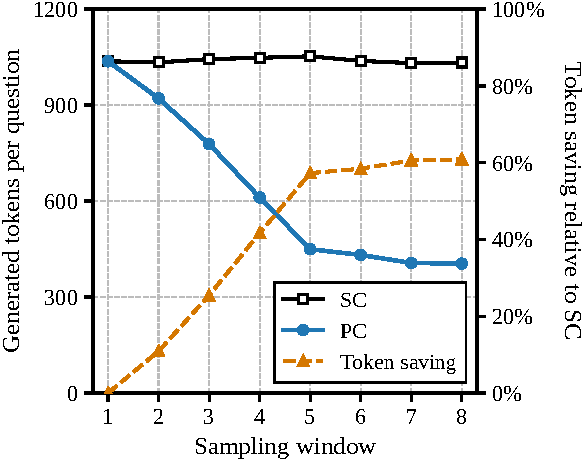
\includegraphics[width=\linewidth]{figs/window_tokens.pdf}
\caption{Tokens and savings by window.}
\label{fig:windows}
\end{minipage}
\end{figure}

Table~\ref{tab:prefix_levels} relates the extent of prefix reuse to the cost of subsequent generation. Windows are grouped by the nominal prefix level used, with level 0 including returns to the empty prefix. Prefix length counts one shared prefix, while generated tokens sum the four continuations per question. Across levels 1 to 4, mean prefix length increases from 39.4 to 177.5 tokens and generated tokens decrease from 859.3 to 256.7 per window. Relative to matched self-consistency windows, token savings rise from 14.3\% to 73.3\%, accompanied by generation-time reductions of 13.4\% to 73.6\%. Thus, higher prefix levels are associated with less remaining generation and larger measured savings.

Figure~\ref{fig:windows} shows how these savings develop over successive sampling windows, averaging over all 1,319 questions. Both methods start from the same unprefixed window. As shared prefixes extend, mean generated tokens under path-consistency decline from 1,036.8 in window 1 to 404.5 in window 8, whereas self-consistency remains near 1,040 tokens per window. The corresponding token saving reaches 60.9\% in the final window. By that point, 89.5\% of questions use a prefix, and mean prefix length across all questions reaches 158.6 tokens. Unlike the level-based groups in Table~\ref{tab:prefix_levels}, this window-level view includes questions at different prefix levels and those without a prefix.

Table~\ref{tab:prefix_case} illustrates the same progression through actual generated text. In this example, the shared prefix grows from 0 to 79 tokens over five windows. By the fourth window, it already contains the calculation of half of Haley's age, so later generation can continue from that intermediate result. By the fifth window, only the remaining subtraction and final answer need to be generated, using 26 tokens compared with 94 in the initial displayed trajectory. The expanding black prefix and shorter blue continuation make the source of the savings explicit. Together, the aggregate results and the example show how reusing intermediate reasoning reduces the generation required by later trajectories.

\begin{table}[t]
\centering\small
\caption{Progressive prefix reuse on a GSM8K example with Llama-3.1-8B-Instruct. Black text is the reused prefix and blue text is newly generated. One recorded trajectory is shown per window.}
\label{tab:prefix_case}
\begin{tabularx}{\linewidth}{@{}X@{}}
\toprule
\textbf{Question.} Geb is 10 less than half the age of Haley. If Haley is 26 years old, how old is Geb? \\
\midrule
\textbf{Window 1, prefix level 0\%} \hfill 0 prefix tokens; 94 generated tokens \\
{\color{blue}To find Geb's age, we need to follow these steps:  1. First, we find half of Haley's age. Haley is 26 years old, so half of her age would be 26 / 2 = 13.  2. Next, we need to subtract 10 from this half age to find Geb's age. So, 13 - 10 = 3.  Therefore, Geb is 3 years old.  $\boxed{3}$} \\
\midrule
\textbf{Window 2, prefix level 20\%} \hfill 17 prefix tokens; 104 generated tokens \\
To find Geb's age, we need to follow these steps:  1. First,\ {\color{blue} we need to find half of Haley's age. Haley is 26 years old, so half of 26 is 26 / 2 = 13.  2. Since Geb is 10 less than half the age of Haley, we need to subtract 10 from the half of Haley's age. So, Geb's age is 13 - 10.  3. Now, let's calculate 13 - 10 = 3.  Therefore, Geb is 3 years old.  $\boxed{3}$} \\
\midrule
\textbf{Window 3, prefix level 40\%} \hfill 34 prefix tokens; 75 generated tokens \\
To find Geb's age, we need to follow these steps:  1. First, we need to find half of Haley's age. Haley is 26 years old,\ {\color{blue} so half of her age would be 26 / 2 = 13.  2. Now that we have half of Haley's age, we need to subtract 10 from this number to find Geb's age.   3. So, Geb's age would be 13 - 10 = 3.  Therefore, Geb is $\boxed{3}$ years old.} \\
\midrule
\textbf{Window 4, prefix level 60\%} \hfill 52 prefix tokens; 56 generated tokens \\
To find Geb's age, we need to follow these steps:  1. First, we need to find half of Haley's age. Haley is 26 years old, so half of her age would be 26 / 2 = 13.  2.\ {\color{blue} Since Geb is 10 less than half the age of Haley, we need to subtract 10 from the half of Haley's age. So, Geb's age would be 13 - 10 = 3.  Therefore, Geb is $\boxed{3}$ years old.} \\
\midrule
\textbf{Window 5, prefix level 80\%} \hfill 79 prefix tokens; 26 generated tokens \\
To find Geb's age, we need to follow these steps:  1. First, we need to find half of Haley's age. Haley is 26 years old, so half of her age would be 26 / 2 = 13.  2. Since Geb is 10 less than half the age of Haley, we need to subtract 10 from the half of Haley's age.\ {\color{blue} So, 13 - 10 = 3.  Therefore, Geb is 3 years old.  $\boxed{3}$} \\
\bottomrule
\end{tabularx}
\end{table}


\subsection{Main results}
\label{sec:main_results}
\begin{table}[htbp]
\centering
\caption{Accuracy and token cost of long-chain reasoning with thinking enabled. PC uses the default $C=0.8$. Tokens are means per question; negative entries in Save indicate reductions relative to SC. MATH-500 accuracy is raw grading on 490 evaluated questions plus ten held-out engineering items counted as correct ($n=500$). Qwen/MATH-500 reports 199 evaluated questions and does not use this $n=500$ convention. DeepSeek GSM8K records are documented in Appendix~\ref{app:threshold}.}
\label{tab:main}
\setlength{\tabcolsep}{5pt}
\begin{tabular}{llcccccc}
\toprule
Model & Dataset & \multicolumn{3}{c}{Accuracy (\%)} & \multicolumn{3}{c}{Tokens (\# per problem)}\\
\cmidrule(lr){3-5}\cmidrule(lr){6-8}
 & & Pass@1 & SC & PC & SC & PC & Save (\%)\\
\midrule
DeepSeek-V4-Flash  & GSM8K & 96.74 & 96.82 & 96.82 & 12,514 & 8,230 & -34.2 \\
& MATH-500 & 86.60 & 88.00 & 87.60 & 41,166 & 26,968 & -34.5 \\
 & AIME 2024 & 93.33 & 96.67 & 96.67 & 288,230 & 213,162 & -26.0 \\
 & AIME 2025 & 86.67 & 100.00 & 100.00 & 351,230 & 260,523 & -25.8 \\
 & GPQA-D & 83.33 & 89.90 & 89.90 & 309,325 & 221,526 & -28.4 \\

\midrule
Qwen3-30B-A3B & GSM8K & 96.59 & 96.74 & 96.59 & 57,859 & 33,564 & -42.0 \\
& MATH-500 & 93.97 & 94.47 & 94.47 & 156,956 & 92,106 & -41.3 \\
 & AIME 2024 & 73.33 & 83.33 & 83.33 & 443,797 & 261,149 & -41.2 \\
 & AIME 2025 & 73.33 & 83.33 & 83.33 & 559,278 & 360,577 & -35.5 \\
 & GPQA-D & 61.76 & 62.94 & 62.35 & 234,446 & 152,079 & -35.1\\
\bottomrule
\end{tabular}
\end{table}

Table~\ref{tab:main} evaluates DeepSeek-V4-Flash and Qwen3-30B-A3B, both generating long reasoning chains with thinking enabled. Across the ten reported settings, path-consistency reduces generated tokens by 25.8\% to 42.0\%, averaging 34.4\% with equal weight assigned to each setting, while largely maintaining voting accuracy.

DeepSeek matches self-consistency's accuracy on GSM8K, both AIME benchmarks, and GPQA-D, and remains within 0.40 percentage points on MATH-500, with an average token saving of 29.8\%. Qwen achieves larger relative savings on every benchmark, averaging 39.0\%, with matching accuracy on MATH-500 and both AIME benchmarks and closely comparable accuracy on GSM8K and GPQA-D. Thus, the efficiency benefit appears across both models rather than being confined to a single setting.

Both models also retain gains over Pass@1 on the AIME benchmarks, showing that reduced generation cost need not eliminate the benefit of multiple sampled paths. Together with Section~\ref{sec:llama}, these results support prefix reuse for both shorter reasoning traces and long thinking chains as a way to reduce token cost while retaining the benefits of answer aggregation.

\subsection{Comparisons and composition}
\label{sec:composition}
Table~\ref{tab:composition} compares path-consistency with reasoning-sharing methods and evaluates its combination with early-stopping methods on Llama-3.1-8B-Instruct and GSM8K. Self-consistency with a reduced budget of $B=20$ provides an additional comparison at a similar token cost. The combinations retain the stopping and aggregation rules of adaptive-consistency and early-stopping self-consistency, so their additional savings are measured relative to each method without prefix reuse.

\begin{table}[htbp]
\centering\small
\caption{Method comparisons and early-stopping combinations on Llama-3.1-8B-Instruct/GSM8K. Tokens are means per question; negative entries in Save indicate reductions relative to SC with $B=32$. The maximum trajectory budget is 32 unless otherwise indicated. Indented rows add PC to the preceding method.}
\label{tab:composition}
\begin{tabular}{lrrr}
\toprule
Method & Accuracy (\%) & Tokens & Save (\%)\\
\midrule
Self-consistency & 92.12 & 8,316 & - \\
Self-consistency ($B=20$) & 91.28 & 5,214 & -37.3\% \\
PoLR ($L_p=128$) & 92.19 & 5,863 & -29.5\% \\
CPT (32 workers) & 92.80 & 8,411 & +1.1\% \\
Path-consistency & 91.74 & 5,039 & -39.4\% \\
\midrule
Adaptive-consistency ($\tau=0.95$) & 92.04 & 4,035 & -51.4\% \\
 \quad + Path-consistency & 92.27 & 3,003 & -63.9\% \\
Early-stopping self-consistency & 92.49 & 4,299 & -48.3\% \\
 \quad + Path-consistency & 92.27 & 3,501 & -57.9\% \\
\bottomrule
\end{tabular}
\end{table}

Path-consistency reduces generated tokens by 39.4\% relative to self-consistency while largely maintaining accuracy. Compared with simply reducing the trajectory budget to 20, it achieves higher accuracy with fewer tokens, supporting prefix reuse as an alternative to discarding sampling opportunities. Among the reasoning-sharing methods, path-consistency uses 14.1\% fewer tokens than PoLR, with closely comparable accuracy. CPT achieves the highest accuracy in this comparison but generates slightly more tokens than self-consistency. These results place path-consistency at a lower token cost rather than establishing uniform superiority across both accuracy and efficiency.

Prefix reuse also complements early stopping. Combined with adaptive-consistency, it reduces mean tokens from 4,035 to 3,003, an additional 25.6\% saving, while accuracy increases from 92.04\% to 92.27\%. Combined with early-stopping self-consistency, it reduces mean tokens from 4,299 to 3,501, an additional 18.6\% saving, while largely maintaining accuracy. Thus, path-consistency reduces generation cost both as a standalone reasoning-sharing method and in combination with early-stopping methods, providing further savings of 18.6\% to 25.6\% over the latter in this evaluation.

\subsection{Ablation studies}
\label{sec:ablations}
\paragraph{Contributions of prefix selection and recovery.}
Table~\ref{tab:selrec} examines local confidence selection and recovery on DeepSeek-V4-Flash/MATH-500 by replacing the selector with uniform selection, disabling recovery, or combining both changes. All configurations use the same 490 evaluated questions and shared self-consistency roots. Accuracy counts the ten held-out engineering items as correct ($n=500$). The remaining settings are fixed; implementation details are given in Appendix~\ref{app:ablation_design}.

\begin{table}[htbp]
\centering\small
\caption{Effects of prefix selection and recovery on DeepSeek-V4-Flash/MATH-500. Accuracy uses raw grading on 490 evaluated questions plus ten held-out engineering items counted as correct ($n=500$). $\Delta$ and Save denote the accuracy difference in percentage points and token reduction relative to SC. Tokens are means per evaluated question.}
\label{tab:selrec}
\begin{tabular}{lrrrr}
\toprule
Method & Accuracy (\%) & $\Delta$ (pp) & Tokens & Save (\%)\\
\midrule
SC & 88.00 & 0.00 & 41,166 & 0.0 \\
\midrule
PC (full) & 87.60 & $-0.40$ & 26,968 & 34.5 \\
\quad w/ uniform selection & 87.20 & $-0.80$ & 25,680 & 37.6 \\
\quad w/o recovery & 86.60 & $-1.40$ & 24,757 & 39.9 \\
\quad w/ uniform selection, w/o recovery & 86.60 & $-1.40$ & 25,405 & 38.3 \\
\bottomrule
\end{tabular}
\end{table}

The full configuration achieves the highest accuracy among the path-consistency variants at 87.60\%, while saving 34.5\% of generated tokens. Uniform selection lowers accuracy to 87.20\%, and disabling recovery lowers it to 86.60\% under either selector. The variants save more tokens, but at the cost of lower accuracy. These results support retaining both components when accuracy preservation is prioritized, with recovery showing the larger observed contribution in this setting.

\paragraph{Sensitivity to the agreement threshold.}
Table~\ref{tab:threshold} examines the trade-off between accuracy and token savings across agreement thresholds on DeepSeek-V4-Flash/GSM8K, with $C=1$ corresponding to self-consistency. The default $C=0.8$ preserves its 96.82\% accuracy while reducing generated tokens by 34.2\%. Lowering $C$ to 0.7 and 0 increases savings to 40.8\% and 43.5\%, respectively, with small accuracy decreases of 0.08 and 0.23 percentage points.

\begin{table}[htbp]
\centering
\caption{Accuracy and token cost across agreement thresholds on DeepSeek-V4-Flash/GSM8K. Tokens are means per question. $\Delta$ and Save report changes relative to SC ($C=1$), with negative Save values indicating token reductions.}
\label{tab:threshold}
\begin{tabular}{lcccc}
\toprule
Threshold ($C$) & Accuracy (\%) & $\Delta$ (pp) & Tokens (\# per problem) & Save (\%)\\
\midrule
1.0 (Self-consistency) & 96.82 & - & 12,514 & - \\
0.8  & 96.82 & 0.00 & 8,230 & -34.2\\
0.7  & 96.74 & -0.08 & 7,399 & -40.8\\
0  & 96.59 & -0.23  & 7,070 & -43.5\\
\bottomrule
\end{tabular}
\end{table}

A lower threshold permits prefix reuse under weaker answer agreement, whereas a higher threshold requires stronger agreement and makes reuse more conservative. The threshold therefore offers a direct way to express user priorities. Lower values favor more efficient generation through greater token savings, while higher values favor accuracy preservation.

\section{Conclusion}
Path-consistency reduces repeated reasoning through shared prefixes controlled by answer agreement, prefix selection, and trial and recovery. Our analysis characterizes how prefix reuse affects voting accuracy and bounds voting error under explicit conditional-margin assumptions. Experiments with three models across five reasoning benchmarks show substantial token savings while largely maintaining accuracy, with further savings when combined with early-stopping methods. These results support prefix reuse as a practical way to make multi-path reasoning more efficient.

\paragraph{Limitations.}
Shared prefixes may propagate undetected errors, so answer agreement does not guarantee correctness. Path-consistency aims to preserve accuracy rather than ensure it. Parallelism is limited by the window size, since successive windows depend on earlier outcomes. Local confidence selection also requires output token log probabilities. APIs that do not expose them require a fallback without confidence scores, such as uniform random selection among eligible prefixes.

\section*{Reproducibility Statement}
To support reproduction of our results, Section~\ref{sec:setup} specifies the evaluated models and benchmarks, decoding settings, trajectory budget, sampling window size, agreement threshold, and prefix levels. Appendix~\ref{app:protocol} details the controller transitions, prompting setup, deterministic preprocessing such as GPQA option shuffling, and ablation settings. Token savings and generation-time measurements use the accounting conventions in Appendix~\ref{app:accounting}, including the costs of unprefixed and failed windows. Appendices~\ref{app:proofs} and~\ref{app:additional_math} provide proofs and additional theoretical analysis. The supplementary materials include runnable code for the API experiments, pinned software dependencies, and instructions for setting up the Python environment and running the implementation and evaluation of path-consistency.

\section*{AI Use Statement}
This revision used OpenAI Codex to inspect the provided manuscript and reviews, assist with theoretical reformulation and English drafting, write aggregation code, and check LaTeX compilation. Existing DeepSeek format-regrading artifacts include model-assisted answer-equivalence judgments, as described in Appendix~\ref{app:grading}. Author verification of the mathematical arguments, grading decisions, references, and final claims remains pending in this working draft. This statement records assistance used; it does not assert that human verification has already occurred.

\section*{Ethics and Data Availability}
The experiments use existing reasoning benchmarks. GPQA question text and API credentials are excluded from the manuscript package. Dataset use and redistribution remain subject to the original providers' terms. Confidence scores should not be interpreted as correctness certificates in downstream high-stakes applications. Author contributions, funding, and competing-interest declarations must be supplied by the authors before finalization.

\bibliography{reference}
\bibliographystyle{iclr2027_conference}
\clearpage
\appendix
\newpage
\renewcommand{\floatpagefraction}{0.9}
\noindent
The appendix provides proofs and additional analysis in Appendices~\ref{app:proofs} and~\ref{app:additional_math}, evaluation details in Appendix~\ref{app:protocol}, and sentence-level prefix experiments in Appendix~\ref{app:sentence}.

\section{Proofs and finite-budget analysis}
\label{app:proofs}
\subsection{Proof of Theorem~\ref{thm:decomposition}}
Define the self-consistency continuation value at any history by backward recursion.
\[
 V_j^S(h)=\int V_{j+1}^S(h,u)K_j^S(du\mid h),\qquad
 V_J^S(h)=\ind\{\text{final vote in }h\text{ is correct}\}.
\]
The notation $(h,u)$ includes the deterministic bookkeeping after the next window. Under path-consistency, conditional expectation gives
\[
 \E_P[V_{j+1}^S(H_{j+1})-V_j^S(H_j)\mid H_j=h]=d_j(h).
\]
Taking expectations and summing over $j$ telescopes. The initial value is $A_S$ and the expected terminal value is $A_P$, proving Equation~\ref{eq:risk}. This argument needs only bounded measurable values and a finite horizon. It does not require independent windows, a binary answer distribution, or a correct selected prefix. Since $0\leq V_{j+1}^S\leq1$, the standard variational definition
\[
 \TV(P,Q)=\sup_{0\leq f\leq1}|\E_Pf-\E_Qf|
\]
implies $|d_j(h)|\leq\TV(K_j^P,K_j^S)$. The triangle inequality and the fact that two probabilities differ by at most one prove Equation~\ref{eq:tv}.

\paragraph{Scope for stopping controllers.}
The displayed result compares fixed-budget self-consistency and path-consistency. A stopping controller can be represented by an absorbing terminal state and padding to a common finite maximum horizon. Both the reference value and the reference transition kernel must then include that parent's stopping rule. This extension does not allow replacing a confidence-weighted parent's final vote by a majority vote while claiming to compare the same parent.

\subsection{Proof of Theorem~\ref{thm:plurality}}
Fix a competitor $a$. The differences $D_i=X_i(a)-\mu_i(a)$ are martingale differences. Conditional on $\mathcal F_{i-1}$, their values lie in an interval of width at most two, since $X_i(a)\in[-1,1]$. The conditional bounded-variable exponential inequality therefore gives
\[
 \E[\exp(-\lambda D_i)\mid\mathcal F_{i-1}]\leq\exp(\lambda^2/2),\quad \lambda>0.
\]
This inequality follows by the convex upper bound on the exponential between the two interval endpoints and maximizing over a zero-mean two-point distribution. Iterating conditional expectations yields
$\E\exp(-\lambda\sum_iD_i)\leq\exp(B\lambda^2/2)$.
If the correct answer fails to outvote $a$, then $\sum_iX_i(a)\leq0$. By the almost-sure lower bound on accumulated conditional means, this implies $\sum_iD_i\leq-\Gamma_a$. Markov's inequality now bounds its probability by
\[
 \exp(-\lambda\Gamma_a+B\lambda^2/2).
\]
Taking $\lambda=\Gamma_a/B$ gives $\exp(-\Gamma_a^2/(2B))$. If the final vote is incorrect or tied, at least one incorrect category has count no smaller than the correct category. Union-bounding these events proves the result. Voting failure is covered by the union of competitor events.

\paragraph{What the assumption rules out.}
An unconditional gap $P(A_i=a^\star)>P(A_i=a)$ is insufficient. Conditioning on an early misleading prefix may reverse the gap, violating the almost-sure lower bound. Similarly, the observed mode need not equal $a^\star$. The Beta gate operates on the mode, whereas the theorem refers to the externally defined correct answer. An empirical evaluation of the assumption needs correctness information and conditional resampling beyond the current trajectories.

\subsection{Exact binary illustration without Taylor expansion}
For comparison with a single-promotion analysis, suppose $n$ root answers are independent Bernoulli with correctness probability $p_0$, and the remaining $r=B-n$ answers are conditionally independent with correctness probability $q_k$ after observing $k$ correct root answers. Fix a tie-as-failure convention. Define
\[
 Q_r(p,t)=\sum_{j=\max(0,t)}^r \binom{r}{j}p^j(1-p)^{r-j},
\]
with $Q_r(p,t)=0$ for $t>r$ and $Q_r(p,t)=1$ for $t\leq0$. Then
\begin{align}
 A_{\mathrm{PC}}&=\sum_{k=0}^{n}\binom{n}{k}p_0^k(1-p_0)^{n-k}
       Q_r(q_k,\lfloor B/2\rfloor+1-k),\label{eq:exactbinary}\\
 A_{\mathrm{SC}}&=Q_B(p_0,\lfloor B/2\rfloor+1).
\end{align}
Both parts contribute to the final vote. A gate that does not promote sets $q_k=p_0$ for that history. The formula is exact for this idealized model, including its tie convention; it is not a model of all levels of path-consistency.

For a concrete failure construction take $B=32,n=4,p_0=0.6,C=0.8$. If the four root answers are all wrong, their agreement score is $1-2^{-5}=0.96875$. Let the selected wrong prefix force all subsequent answers to be wrong ($q_0=0$), while all other histories retain $q_k=0.6$. The accuracy loss relative to self-consistency is exactly
\[
 (0.4)^4 Q_{28}(0.6,17)>0.
\]
Numerically, self-consistency accuracy in this construction is 0.835203095 and the intervention accuracy is 0.821096895, a loss of 1.41 percentage points. Thus even a model whose unprefixed correctness probability exceeds one half can be harmed by a gate-passing prefix. The construction does not assume symmetric beneficial and harmful effects. That symmetry is an additional modeling assumption, not an inference-time property. More generally, a consensus-only controller has no access to the sign of a prefix's correctness effect.

\subsection{Shared-prefix dependence}
Let a random shared prefix $Z$ induce correctness probability $p_Z$, and let $Y_1,Y_2$ be correctness indicators of two suffixes that are conditionally independent given $Z$. Then $\E[Y_1Y_2\mid Z]=p_Z^2$ and $\E Y_i=\E p_Z$, so
\begin{equation}
 \operatorname{Cov}(Y_1,Y_2)=\operatorname{Var}(p_Z).
 \label{eq:dependence}
\end{equation}
For a window of size $m$ with exchangeable correctness indicators, marginal correctness probability $\bar p$, and pairwise correlation $\rho$, summing variances and covariances gives
\[
 \operatorname{Var}(\bar Y)=\frac{\bar p(1-\bar p)}{m}[1+(m-1)\rho].
\]
For $0<\bar p<1$ and a positive variance inflation factor, this corresponds to $m/[1+(m-1)\rho]$ independent Bernoulli observations with the same variance. This conditional-mixture illustration is not an estimate of the effective sample size of a full path-consistency run. Neither that value nor a plug-in correction is used to calibrate the actual path-consistency gate.

\section{Additional analysis of prefix reuse}
\label{app:additional_math}
The following results clarify when prefix reuse can affect the final vote and how shared prefixes change the relationship between trajectory accuracy and voting accuracy.

\subsection{When can later windows still change the vote?}
Let $c_a$ count all valid votes for answer $a$ already generated, including votes from rejected windows. Let $\ell$ be a unique current leader and let $r$ be an upper bound on the number of answers still to be generated. Include an unseen competitor with count zero when defining $c_{(2)}=\max_{a\ne\ell}c_a$. Each remaining trajectory supplies at most one unit vote, and earlier votes cannot be removed or reweighted.

\begin{proposition}[Irreversible plurality]
\label{prop:lock}
If $c_\ell-c_{(2)}>r$, then $\ell$ is the unique final plurality winner for every possible continuation, including adaptive and dependent continuations. If $c_\ell-c_{(2)}<r$, a continuation assigning every remaining vote to a strongest competitor can overturn the leader. At equality a competitor can tie, so the outcome depends on the fixed tie rule.
\end{proposition}
\begin{proof}
For any competitor, the largest possible increase in its count relative to the leader is $r$. Thus its final deficit is at least $c_\ell-c_a-r$. A strictly positive minimum guarantees the leader remains unique. Conversely, giving all $r$ votes to a strongest competitor realizes that maximum increase, proving the remaining statements. Invalid outputs can only reduce the number of added votes and cannot break the sufficient condition.
\end{proof}

The statement concerns the realized vote, not correctness. Once a wrong leader is locked, a rollback cannot repair the final answer under this aggregation rule. Once a correct leader is locked, later prefixes cannot change final correctness either. For a fixed $B=32,m=4$, one may test the sufficient condition after window $j$ using $r=32-4j$. This is a diagnostic of the final vote, not a stopping rule used in the experiments. The condition says only that later votes cannot alter the outcome; it does not undo any effect of earlier prefixes on the current counts.

There is also a useful consequence for Theorem~\ref{thm:decomposition}. On a locked history, $V^S$ is constant over all admissible next windows, so $d_j(h)=0$. Accordingly,
\[
 |A_P-A_S|\leq\min\left\{1,\sum_j\E_P\left[
 \ind\{H_j\text{ is not locked}\}\,
 \TV(K_j^P(\cdot\mid H_j),K_j^S(\cdot\mid H_j))\right]\right\}.
\]
This refinement localizes possible final-vote effects to histories where future votes can still matter. It does not assert that unlocked histories are recoverable under the model's actual support, nor that their increments are favorable.

\subsection{Higher marginal correctness can yield a worse majority}
For a binary illustration, condition on a history with $n$ earlier votes, $k$ of them correct, and $r=B-n$ remaining votes. A random shared prefix $Z$ induces a correctness probability $p_Z$; conditional on $Z$ and the history, the remaining answers are independent Bernoulli variables. With ties counted as failures, let $t=\lfloor B/2\rfloor+1-k$. Using the binomial tail from Equation~\ref{eq:exactbinary}, the conditional final success probability is
\begin{equation}
 A_{\mathrm{shared}}(h)=\E[Q_r(p_Z,t)\mid h].
 \label{eq:mixturevote}
\end{equation}
If an independent prefix were instead drawn for each remaining answer under this stylized model, the probability would be $Q_r(\bar p,t)$, where $\bar p=\E[p_Z\mid h]$. These two expressions generally differ even at identical marginal correctness. Independent-prefix resampling here is an analytical comparator, not an evaluated path-consistency variant.

\begin{proposition}[Curvature of the voting response]
For $1\leq t\leq r$ and $0<p<1$,
\[
 \frac{d Q_r(p,t)}{dp}
 =r\binom{r-1}{t-1}p^{t-1}(1-p)^{r-t},
\]
and the sign of its second derivative is the sign of
$(t-1)-(r-1)p$. Thus $Q_r$ is concave above $p=(t-1)/(r-1)$ and convex below it when $r>1$. If the support of $p_Z$ lies wholly in the concave region, sharing cannot improve the voting probability relative to independent resampling at the same mean; in the convex region the inequality reverses.
\end{proposition}
\begin{proof}
Differentiate the finite binomial sum. Adjacent terms cancel, leaving the stated first derivative. Its logarithmic derivative is $(t-1)/p-(r-t)/(1-p)$, which has the stated sign. Jensen's inequality on either curvature region gives the comparison. For $r=1$ the response is linear. For $t\leq0$ or $t>r$ it is constant. When the support crosses the inflection point, these local curvature statements imply no universal ordering.
\end{proof}

For a finite-budget counterexample retaining the root votes, take four independent root answers with correctness probability 0.6 and 28 later answers sharing a latent prefix. Independently of the root, let $p_Z=1$ with probability 0.65 and $p_Z=0$ otherwise. The final vote is correct exactly when $p_Z=1$, hence its accuracy is 0.65. In contrast, 32 independent answers with correctness probability 0.6 succeed with probability $Q_{32}(0.6,17)=0.835203095$. Every later answer in the shared construction has higher marginal correctness (0.65 versus 0.6), and the mean across all 32 is 0.64375, yet its majority is worse. This deliberately extreme mixture is not a fitted path-consistency model or an assertion that these prefixes occur in the experiments. It demonstrates why per-trajectory correctness and agreement alone do not identify the accuracy of a shared-prefix vote.


\subsection{Agreement thresholds under a fixed answer distribution}
\label{app:gate_analysis}
A fixed-distribution calculation helps distinguish evidence for answer concentration from evidence for correctness. Suppose $n$ answers are sampled independently from one distribution with correct-answer probability $q$. For $1/2<C<1$, define
\[
 k_C(n)=\min\{k\in\{0,\ldots,n\}:c(n,k)\geq C\},
\]
taking $k_C(n)=n+1$ when the set is empty. The score in Equation~\ref{eq:beta} is increasing in $k$, and $k_C(n)>n/2$. Hence the correct answer passes the gate exactly when its count reaches $k_C(n)$, with probability
\[
 \Prb(\text{correct answer passes})=Q_n(q,k_C(n)).
\]
This expression concerns the source answer, not the semantic correctness of every token in its prefix.

An incorrect answer can pass only if the total number of incorrect answers is at least $k_C(n)$. Therefore
\[
 \Prb(\text{an incorrect answer passes})
 \leq Q_n(1-q,k_C(n)).
\]
Equality holds when all incorrect probability mass is concentrated on one alternative. This identifies a worst-case error distribution for a single fixed-distribution check. Raising $C$ increases the required count and reduces both correct and incorrect gate-passing probabilities at that check. In particular, a majority of correct answers can still fail a stringent gate, so the probability of failing to pass cannot be bounded solely by the probability of lacking a correct majority.

Successive checks in path-consistency reuse observations and change the sampling distribution. Their error probabilities therefore cannot be multiplied as if the checks were independent. More generally, if the conditional probability of an incorrect gate-passing decision at check $j$, given its preceding history, is bounded by $\varepsilon_j$, the probability of any such decision is at most $\sum_j\varepsilon_j$ by a union bound and conditional expectation. The gate itself does not establish these conditional bounds. The adaptive analysis in Section~\ref{sec:theory} avoids treating repeated agreement as a correctness guarantee.

\section{Method and evaluation details}
\label{app:algorithm}
\label{app:protocol}
\subsection{Window transitions and answer aggregation}
Table~\ref{tab:state_transitions} summarizes the controller in Section~\ref{sec:method}. The admitted set $\mathcal V$ controls prefix proposals and validation, whereas the final vote uses all valid completed answers. Answers from previously accepted windows remain in $\mathcal V$ after rollback.

\begin{table}[!htbp]
\centering\small
\caption{Prefix updates at window boundaries. Every valid completed answer remains eligible for final aggregation.}
\label{tab:state_transitions}
\begin{tabularx}{\linewidth}{@{}lXX@{}}
\toprule
State & Observation & Update\\
\midrule
Root & Valid answers available & Add answers to $\mathcal V$; propose an extension if the gate passes and a candidate exists.\\
Trial & Same modal answer and $c\geq C$ & Commit the prefix, admit answers, clear the failure count, and consider the next extension.\\
Trial & Modal answer changes or $c<C$ & Discard the proposal, return to the committed prefix, and increment the failure count.\\
Committed & Same modal answer and $c\geq C$ & Retain the prefix, admit answers, clear the failure count, and consider the next extension.\\
Committed & Modal answer changes or $c<C$ & Roll back one level and increment the failure count.\\
Any prefix & Two consecutive failures & Clear the prefix and disable further reuse for this question.\\
\bottomrule
\end{tabularx}
\end{table}

Failed windows provide neither admitted answers nor new prefix candidates. A failed candidate is not permanently excluded from all later source pools. When combined with an early-stopping method, sampling ends at a completed window according to that method's stopping rule, and its aggregation rule is retained.

\subsection{Datasets and prompting}
% Citations needed for the datasets and their official evaluation protocols.
We use the GSM8K test split, MATH-500, AIME 2024, AIME 2025, and GPQA-Diamond. GPQA option order is shuffled deterministically with seed 2027.

The mathematical reasoning instruction is \emph{Please reason step by step, and put your final answer within \texttt{\textbackslash boxed\{\}}.} GPQA presents four labeled options and requests the correct option letter in the same format. Llama uses its chat template. DeepSeek and Qwen use thinking mode, with the decoding settings in Section~\ref{sec:setup}. These interfaces differ, so comparisons are made within each model and dataset.

\subsection{Token and time accounting}
\label{app:accounting}
At an empty prefix, path-consistency reuses the corresponding self-consistency window, including after a return to root. Its original token count and generation time are charged in full. Windows with nonempty prefixes generate new continuations, and failed windows are also counted.

Let $T_{ij}$ and $G_{ij}$ be generated tokens and generation time for window $j$ of question $i$. Over $n$ questions, the means are
\[
 \bar T=\frac{1}{n}\sum_{i,j}T_{ij},\qquad
 \bar G=\frac{1}{n}\sum_{i,j}G_{ij}.
\]
Token savings are $1-\bar T_{\mathrm{PC}}/\bar T_{\mathrm{SC}}$, and a generation speed ratio is $\bar G_{\mathrm{SC}}/\bar G_{\mathrm{PC}}$. Tables with negative Save entries instead display the signed relative token change. A nominal prefix fraction is not a measured saving because continuation lengths can change. These measurements do not include all input-processing and orchestration costs or establish peak-memory and API-billing savings.

\subsection{Ablation settings}
\label{app:ablation_design}
The prefix-selection and recovery ablation fixes the 490 DeepSeek/MATH-500 evaluated questions, self-consistency root windows, source eligibility, prefix-length grid, and decoding settings. Accuracy additionally counts ten held-out engineering items as correct ($n=500$). Uniform selection samples from the same eligible candidates. Disabling recovery retains the active prefix after failure and disables the two-failure reset, while failed-window answers remain excluded from $\mathcal V$. All valid answers still enter the final vote. This removes the recovery mechanism as a whole rather than isolating a single rollback operation.

The full configuration and the three alternatives in Table~\ref{tab:selrec} have 438, 436, 433, and 433 correct answers out of 500. Relative to the full configuration, the alternatives have paired gains/losses of 3/5, 4/9, and 5/10. These single-run differences describe the observed contribution of each component rather than establishing its variability across repeated runs.

\paragraph{Agreement threshold.}
\label{app:threshold}
Table~\ref{tab:threshold} compares $C\in\{0,0.7,0.8,1\}$ on DeepSeek/GSM8K. At $C=0$, the gate imposes no minimum agreement score, but a valid modal answer and feasible prefix are still required. At $C=1$, prefix reuse is disabled. Lower values favor token savings, while higher values make reuse more conservative and favor accuracy preservation. The default remains $C=0.8$; this sensitivity analysis does not identify a universally optimal threshold.

\paragraph{Prefix length at a fixed history.}
\label{app:length_intervention}
A supplementary DeepSeek/MATH-500 study fixes the first-window history and the source chosen by local confidence selection, then varies the retained fraction over $\{0,0.2,0.4,0.6,0.8\}$. It covers 466 questions with feasible prefixes at every level and eight repetitions of a four-answer window per level. Of the remaining questions, 19 do not pass the initial gate and five lack a feasible endpoint. The final-vote diagnostic combines the intervened window with the same four root answers and 24 unprefixed answers. It therefore isolates one window under a fixed continuation, rather than estimating the full continuation expectation in Equation~\ref{eq:risk}. This analysis does not change the fixed prefix-length grid used at inference time.


\section{Initial exploration of sentence-level prefix reuse}
\label{app:sentence}
Before developing the current method, we first explored a sentence-level form of path-consistency for short-chain reasoning. The idea was to reuse complete early reasoning steps rather than generate every trajectory from scratch. This initial approach achieved substantial token savings with generally comparable accuracy on several arithmetic, commonsense, and symbolic tasks, motivating the controlled prefix reuse developed in Section~\ref{sec:method}. We summarize these earlier experiments and the insights they provided below.

The sentence-level approach samples 20 trajectories and randomly selects from eligible prefix candidates ending at sentence boundaries. Its default schedule allows three extension levels, with updates after every five trajectories. Unlike the current method, it does not use one shared prefix per window, the token-fraction grid, or the same trial-and-recovery controller. The results therefore characterize this initial approach and are not pooled with the main experiments.

The Llama-3-8B experiments use temperature 0.6, top-$p=0.9$, few-shot reasoning prompts, and an RTX 3090. Here a prefix level counts retained reasoning steps rather than a fraction of trajectory tokens. Comparisons retain their own self-consistency baselines and timing conventions. Reported speedup percentages denote the increase in speed relative to the corresponding baseline, not the percentage reduction in elapsed time.
% Source: paper/NIPS/04_evaluation.tex, Experimental Setting.
% Citation placeholders for Llama-3, Mistral, DeepSeek-V3, Llama-3.2, datasets, and baseline methods.

\subsection{Arithmetic, commonsense, and symbolic reasoning}
Table~\ref{tab:sentence_tasks} reports our initial results across ten short-chain reasoning tasks~\citep{cobbe2021training, patel2021nlp, miao2020diverse, roy2015solving,geva2021did,suzgun-etal-2023-challenging}. Sentence-level reuse reduces token generation across all tasks and thresholds, with savings ranging from 4.7\% to 36.6\%. Arithmetic accuracy is generally close to or above the self-consistency baseline. At $C=0.8$, GSM8K and Tracking Shuffled Objects improve by 3.7 and 5.2 percentage points, respectively, while Ruin Names and Logical Deduction decline. These results established the practical potential of prefix reuse while showing that its accuracy effects depend on the task.

\begin{table}[!htbp]
\centering\small
\caption{Sentence-level prefix reuse with Llama-3-8B. Each PC entry gives accuracy (\%) / token saving (\%) relative to its SC baseline. These results use the supplementary 20-trajectory setting.}
\label{tab:sentence_tasks}
\setlength{\tabcolsep}{4pt}
\begin{tabular}{@{}lrrrrr@{}}
\toprule
Dataset & SC accuracy (\%) & $C=0$ & $C=0.7$ & $C=0.8$ & $C=0.9$\\
\midrule
\multicolumn{6}{l}{Arithmetic reasoning}\\
GSM8K & 64.1 & 66.6 / 24.0 & 67.1 / 16.1 & 67.8 / 16.2 & 66.6 / 9.9\\
SVAMP & 79.3 & 78.8 / 36.6 & 78.5 / 29.4 & 79.2 / 29.7 & 79.9 / 22.3\\
ASDiv & 81.0 & 80.1 / 32.7 & 81.2 / 27.2 & 80.0 / 27.1 & 80.6 / 22.6\\
MultiArith & 96.7 & 97.8 / 34.8 & 97.2 / 33.3 & 98.9 / 33.1 & 98.3 / 27.2\\
\midrule
\multicolumn{6}{l}{Commonsense reasoning}\\
StrategyQA & 71.4 & 70.8 / 27.8 & 70.6 / 24.0 & 71.3 / 22.1 & 71.1 / 16.0\\
Ruin Names & 76.0 & 71.2 / 9.8 & 74.4 / 7.2 & 72.0 / 6.6 & 71.6 / 4.7\\
Salient Translation & 54.8 & 58.4 / 25.8 & 57.2 / 18.3 & 56.4 / 16.4 & 55.2 / 10.6\\
\midrule
\multicolumn{6}{l}{Symbolic reasoning}\\
Boolean Expressions & 88.4 & 90.0 / 21.3 & 89.6 / 19.8 & 88.8 / 20.3 & 89.6 / 18.3\\
Tracking Shuffled Objects & 54.0 & 58.0 / 16.7 & 56.0 / 12.4 & 59.2 / 10.8 & 58.4 / 6.8\\
Logical Deduction & 78.8 & 76.8 / 26.1 & 78.8 / 20.5 & 77.2 / 24.8 & 76.0 / 17.5\\
\bottomrule
\end{tabular}
\end{table}

\begin{table}[!htbp]
\centering\small
\caption{Reported generation speedups (\%) for the sentence-level experiments in Table~\ref{tab:sentence_tasks}, relative to each task's SC baseline.}
\label{tab:sentence_time}
\begin{tabular}{@{}lrrrr@{}}
\toprule
Dataset & $C=0$ & $C=0.7$ & $C=0.8$ & $C=0.9$\\
\midrule
GSM8K & 28.9 & 18.0 & 17.4 & 10.2\\
SVAMP & 48.3 & 36.6 & 35.7 & 24.8\\
ASDiv & 42.0 & 32.1 & 31.1 & 24.9\\
MultiArith & 42.7 & 40.8 & 40.5 & 33.8\\
StrategyQA & 34.2 & 29.4 & 24.3 & 16.4\\
Ruin Names & 10.4 & 7.8 & 7.4 & 4.7\\
Salient Translation & 30.5 & 19.6 & 17.3 & 10.2\\
Boolean Expressions & 26.6 & 24.3 & 25.2 & 22.0\\
Tracking Shuffled Objects & 18.4 & 12.9 & 11.3 & 6.8\\
Logical Deduction & 31.6 & 23.1 & 30.1 & 19.1\\
\bottomrule
\end{tabular}
\end{table}

Lower thresholds generally permit larger savings, but the trend need not be monotonic after the generated history changes. Logical Deduction, for example, saves more tokens at $C=0.8$ than at $C=0.7$. The smaller improvements on Ruin Names also show that the benefit depends on the task, rather than only on the trajectory budget.

\subsection{Prefix growth and extension frequency}
Table~\ref{tab:sentence_levels} shows how savings grow with sentence-level prefixes on GSM8K. At $C=0.8$, token savings rise from 9.8\% at level 1 to 33.3\% at level 3. This observation motivated progressive prefix extension in the current method, where prefix length is expressed as a fraction of reasoning tokens rather than a number of sentences.

\begin{table}[!htbp]
\centering\small
\caption{GSM8K efficiency by sentence-prefix level. The left group reports speedup (\%); the right group reports token saving (\%), each relative to the corresponding unprefixed baseline.}
\label{tab:sentence_levels}
\begin{tabular}{@{}lrrrrrrrr@{}}
\toprule
& \multicolumn{4}{c}{Speedup (\%)} & \multicolumn{4}{c}{Save (\%)}\\
\cmidrule(lr){2-5}\cmidrule(l){6-9}
$C$ & Overall & Level 1 & Level 2 & Level 3 & Overall & Level 1 & Level 2 & Level 3\\
\midrule
0 & 28.9 & 18.8 & 42.6 & 78.9 & 24.0 & 16.9 & 32.7 & 47.4\\
0.7 & 18.0 & 10.0 & 25.3 & 46.5 & 16.1 & 9.4 & 21.3 & 33.8\\
0.8 & 17.4 & 9.8 & 25.0 & 43.9 & 16.2 & 9.8 & 21.8 & 33.3\\
0.9 & 10.2 & 4.2 & 13.3 & 27.0 & 9.9 & 4.2 & 12.7 & 23.0\\
\bottomrule
\end{tabular}
\end{table}
% Source Table 2 additionally reports token means 96.60 (SC),
% 73.37, 81.09, 80.91, 87.01 (PC). Its averaging unit is not explicit;
% retain the unambiguous relative savings rather than reinterpret these as per-question totals.
% The original speedup.pdf swaps the C=0.7 and C=0.8 level-3 ordering.
% Table values above are authoritative; the inconsistent plot is not reproduced.

With the same 20-trajectory budget, allowing four rather than three extension levels also changes the update interval from five trajectories to four. Table~\ref{tab:sentence_frequency} shows increased savings under the more frequent schedule. Accuracy is unchanged at $C=0.8$ and lower at $C=0.7$. Because depth and update interval change together, this comparison does not isolate the effect of window size.

\begin{table}[!htbp]
\centering\small
\caption{Extension depth and update interval on Llama-3-8B/GSM8K with sentence-level prefixes. Speedup and Save are relative to SC.}
\label{tab:sentence_frequency}
\begin{tabular}{@{}rrrrrr@{}}
\toprule
$C$ & Max. level & Window size & Accuracy (\%) & Speedup (\%) & Save (\%)\\
\midrule
0.7 & 3 & 5 & 67.1 & 18.0 & 16.1\\
0.7 & 4 & 4 & 66.3 & 20.5 & 20.0\\
0.8 & 3 & 5 & 67.8 & 17.4 & 16.2\\
0.8 & 4 & 4 & 67.8 & 18.0 & 17.8\\
\bottomrule
\end{tabular}
\end{table}

\subsection{Method comparisons across model families}
Table~\ref{tab:sentence_models} compares sentence-level prefix reuse with early-stopping methods. On Llama-3-8B, path-consistency uses fewer tokens than either early-stopping baseline on all three tasks, with accuracy between or close to the comparison methods. The DeepSeek-V3 and Llama-3.2-1B-Instruct results show the same cost advantage, but the smaller model loses some accuracy on GSM8K and StrategyQA. Together, these experiments suggested that sentence-level reuse was useful across model families, while its accuracy remained constrained by the quality of the underlying reasoning.

\begin{table}[!htbp]
\centering\small
\caption{Supplementary method comparisons. Entries are accuracy (\%) / mean tokens per question. Each model block is a separate evaluation. AC and ESC denote adaptive-consistency and early-stopping self-consistency. The Llama-3-8B baseline here differs from that in Table~\ref{tab:sentence_tasks}.}
\label{tab:sentence_models}
\begin{tabular}{@{}llrrr@{}}
\toprule
Model & Method & GSM8K & SVAMP & StrategyQA\\
\midrule
Llama-3-8B~\citep{grattafiori2024llama3herdmodels} & SC & 68.4 / 3,860 & 80.4 / 2,321 & 71.7 / 1,805\\
& AC & 67.2 / 2,248 & 79.7 / 935 & 71.2 / 706\\
& ESC & 67.2 / 2,710 & 79.2 / 1,154 & 70.8 / 782\\
& PC & 67.8 / 1,630 & 79.2 / 816 & 71.3 / 700\\
\midrule
DeepSeek-V3~\citep{liu2024deepseek} & AC & 91.6 / 828 & 94.7 / 363 & 84.5 / 326\\
& ESC & 91.6 / 868 & 94.7 / 358 & 84.2 / 315\\
& PC & 91.8 / 786 & 94.7 / 263 & 84.5 / 230\\
\midrule
Llama-3.2-1B-Instruct & AC & 48.1 / 2,748 & 61.1 / 800 & 63.9 / 1,401\\
& ESC & 47.9 / 2,324 & 61.9 / 924 & 63.7 / 1,136\\
& PC & 47.3 / 1,430 & 62.0 / 711 & 63.1 / 799\\
\bottomrule
\end{tabular}
\end{table}

Table~\ref{tab:sentence_mistral} provides another threshold comparison on Mistral-7B. Removing the agreement barrier gives the largest token saving but lower accuracy, while higher thresholds retain accuracy closer to the self-consistency baseline with smaller savings.

\begin{table}[!htbp]
\centering\small
\caption{Sentence-level prefix reuse on Mistral-7B/GSM8K. Speedup and Save are relative to SC.}
\label{tab:sentence_mistral}
\begin{tabular}{@{}lrrrr@{}}
\toprule
Method & $C$ & Accuracy (\%) & Speedup (\%) & Save (\%)\\
\midrule
SC & 1.0 & 59.7 & 0.0 & 0.0\\
PC & 0.0 & 58.5 & 22.0 & 20.3\\
PC & 0.8 & 60.3 & 11.1 & 11.4\\
PC & 0.9 & 60.4 & 6.2 & 6.6\\
\bottomrule
\end{tabular}
\end{table}

\subsection{Token allocation and answer agreement}
\label{app:motivation}
Our initial token analysis in Figure~\ref{fig:historical_motivation} compared generation on trajectories with correct and incorrect final answers. Sentence-level reuse reduces generated text in both groups, supporting the idea that savings come from shortening later continuations rather than only avoiding incorrect answers. Final-answer labels do not identify which individual reasoning tokens are unnecessary. Figure~\ref{fig:overview} complements this analysis by directly visualizing repeated token sequences.

\begin{figure}[!htbp]
\centering
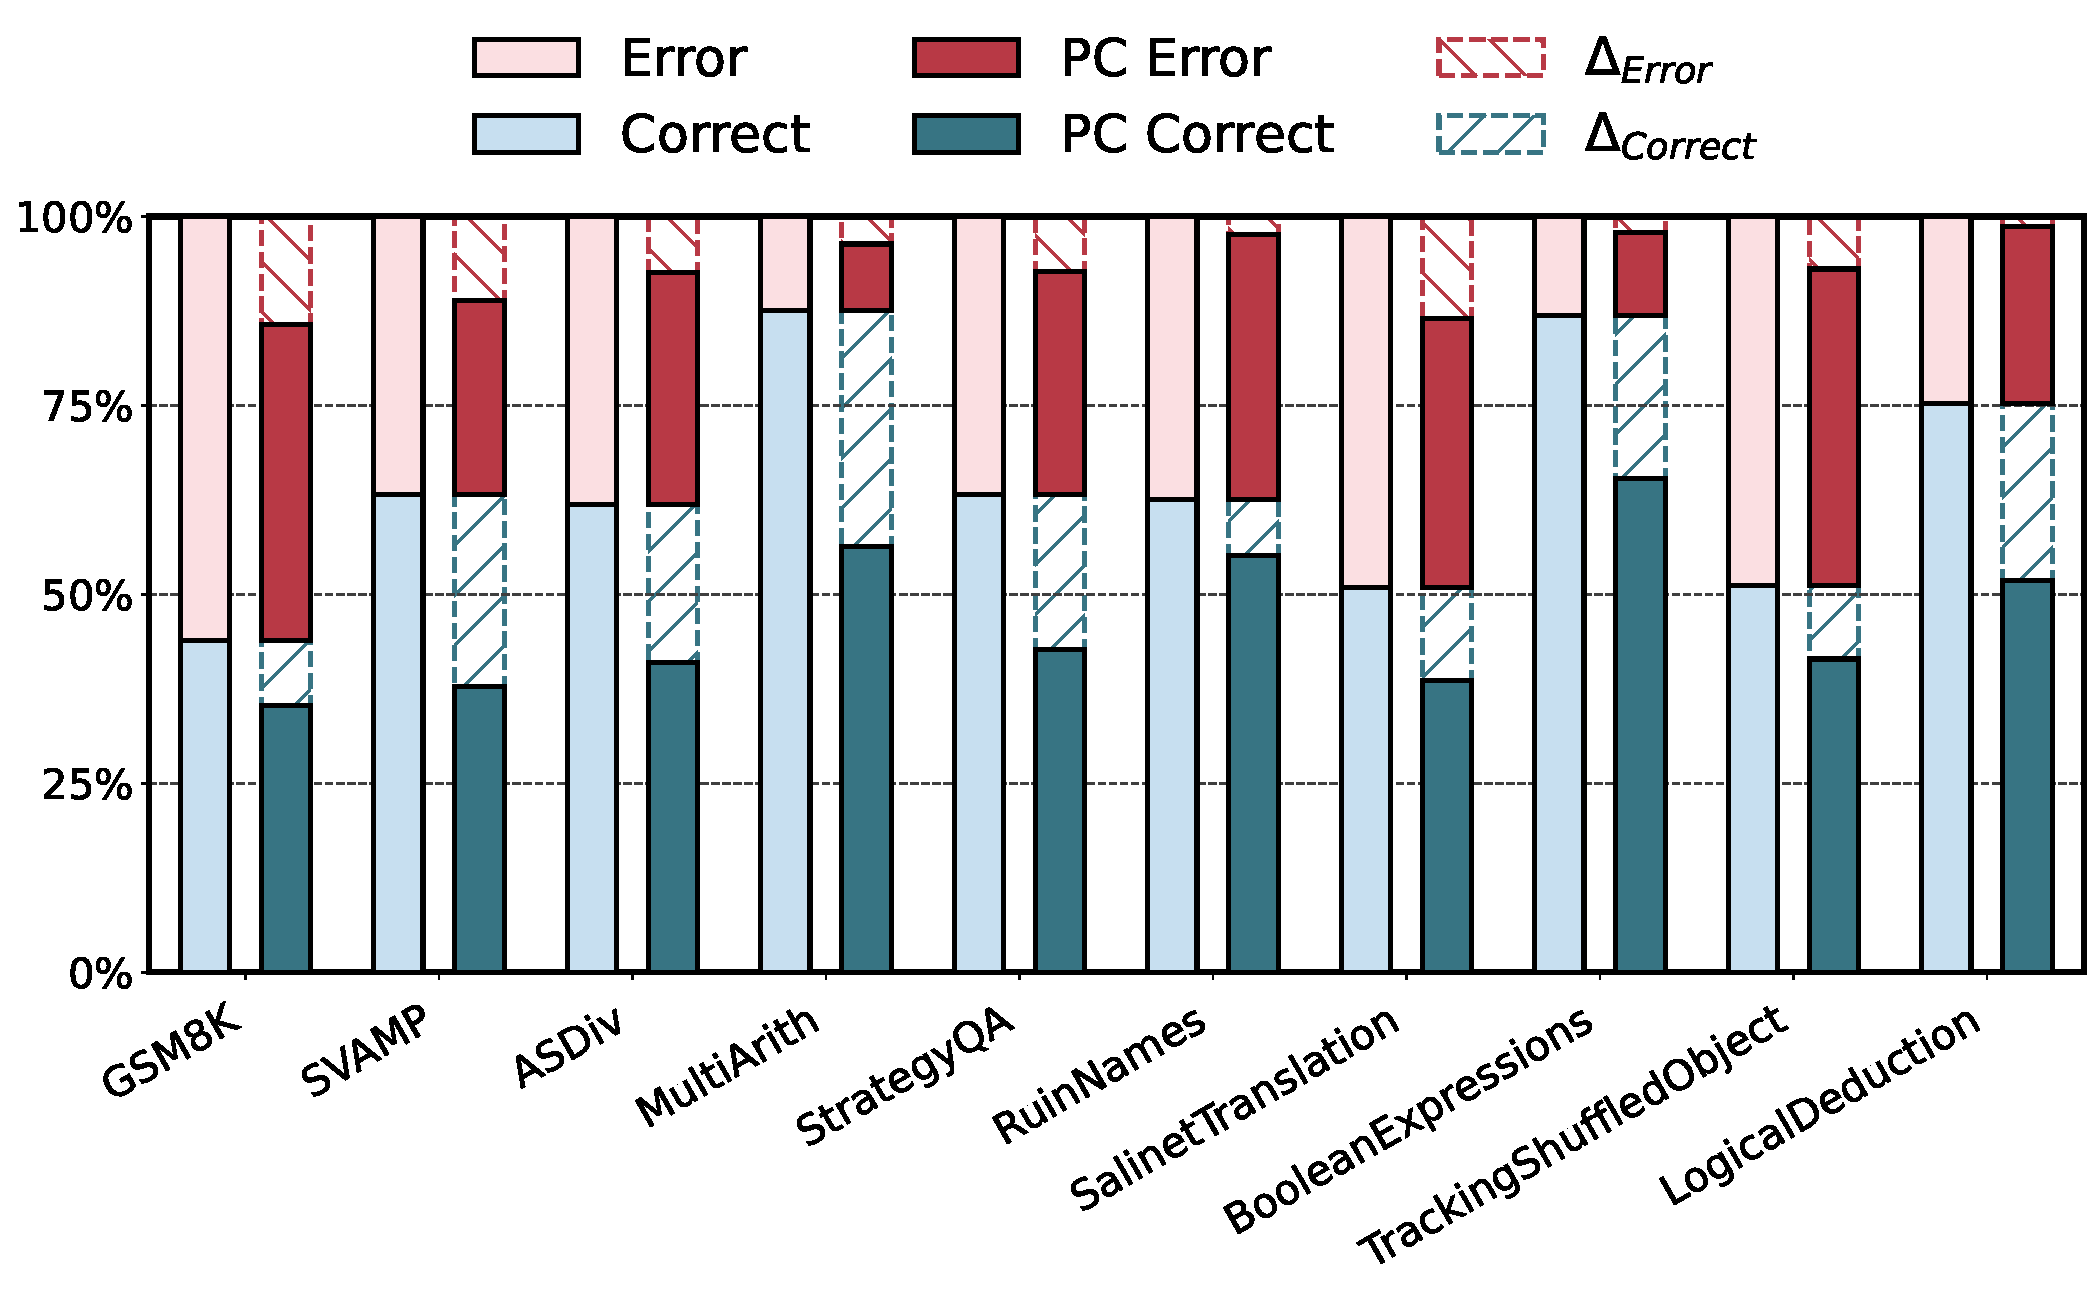
\includegraphics[width=\linewidth]{figs/supp_token_allocation_comparison.pdf}
\caption{Token allocation in the initial sentence-level experiments. Light bars show SC, dark bars show PC, and hatched areas indicate reductions relative to SC. Correct and Error classify trajectories by their final answers, not individual tokens.}
\label{fig:historical_motivation}
\end{figure}

We also examined whether answer agreement could guide prefix reuse. Figure~\ref{fig:sentence_agreement} shows that stronger agreement after ten self-consistency trajectories is associated with correct answers across several tasks. Figure~\ref{fig:sentence_agreement_final} compares the final distributions on GSM8K, where sentence-level reuse produces more concentrated agreement. Incorrect answers nevertheless occur at high agreement. These observations motivated agreement-guided control, but not the interpretation of agreement as a correctness certificate.

\begin{figure}[!htbp]
\centering
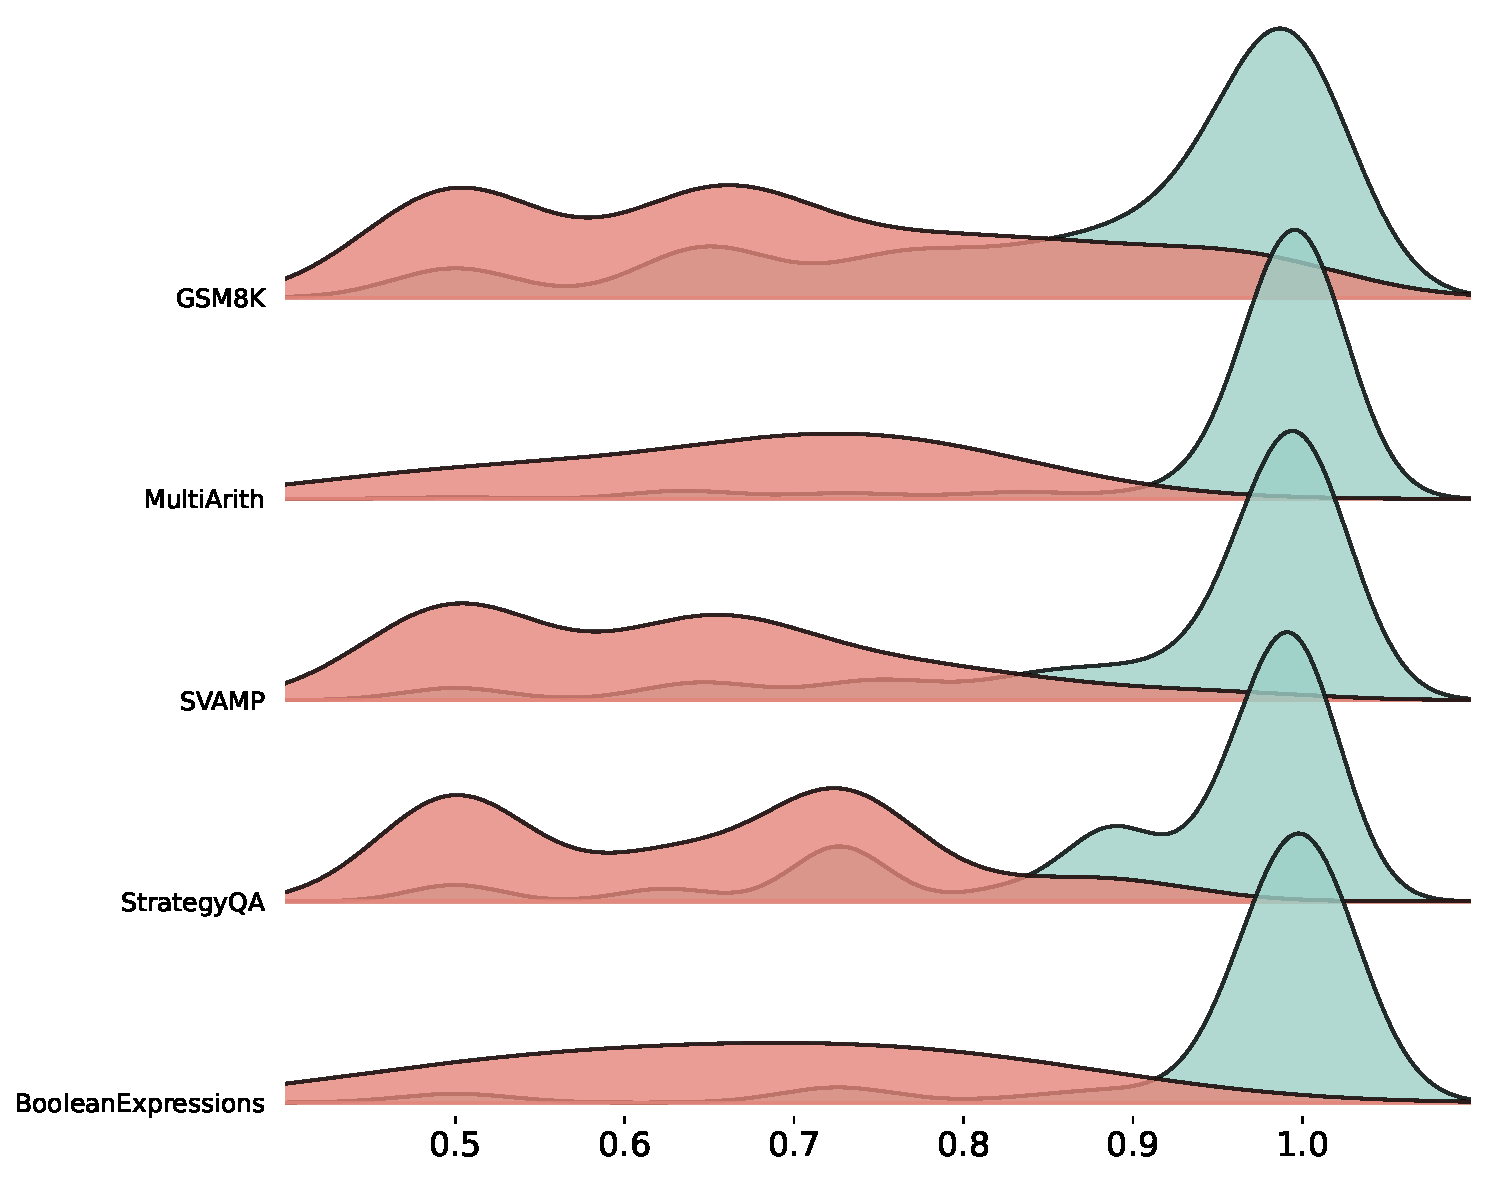
\includegraphics[width=0.62\linewidth]{figs/supp_agreement_by_task.pdf}
\caption{Answer agreement after ten SC trajectories in the initial experiments. Green and red show the distributions for correct and incorrect answers, respectively.}
\label{fig:sentence_agreement}
\end{figure}

\begin{figure}[!htbp]
\centering
\begin{minipage}[t]{0.48\linewidth}
\centering
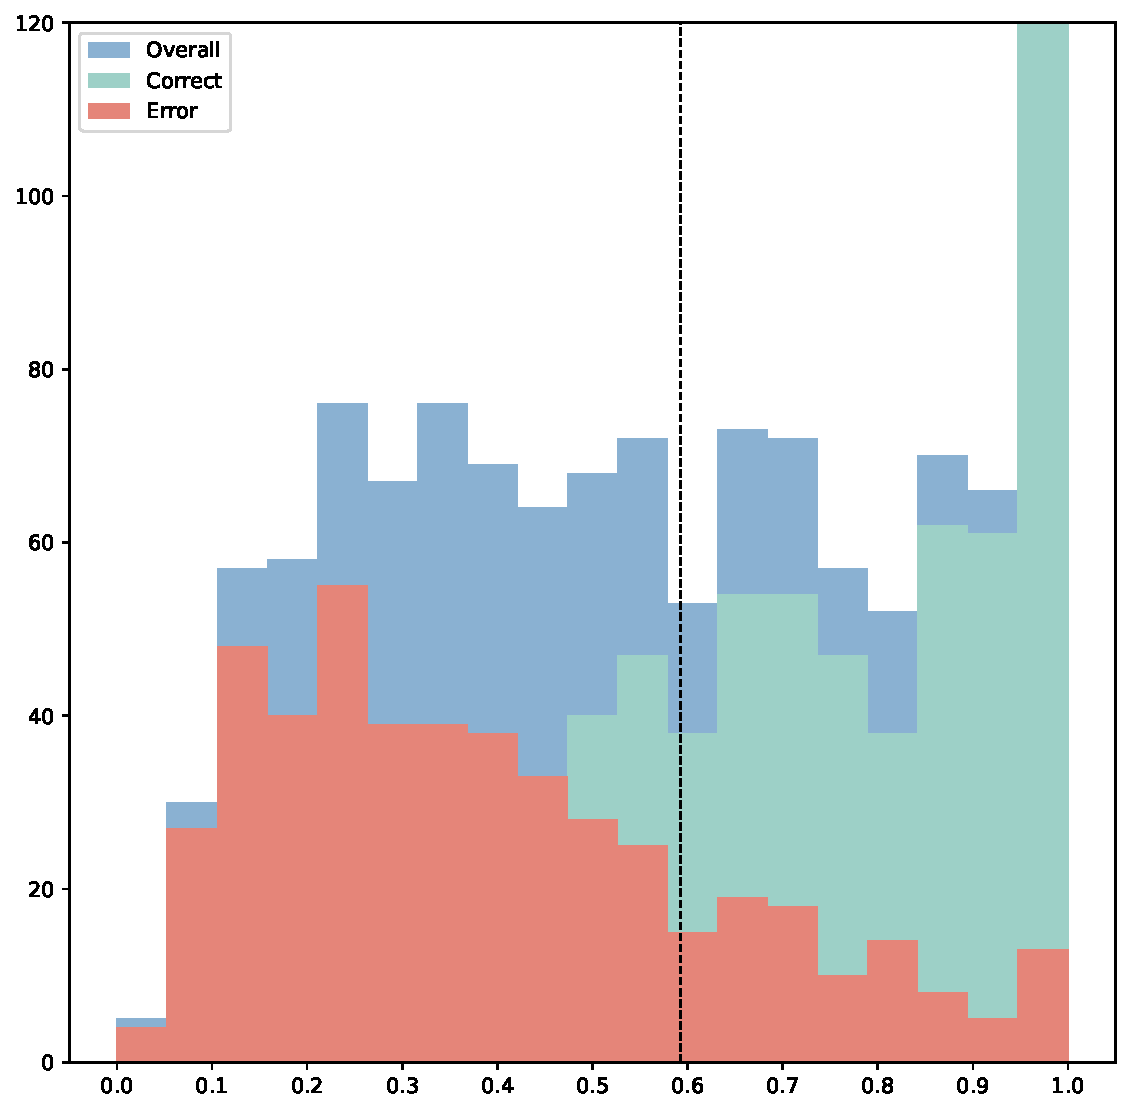
\includegraphics[width=\linewidth]{figs/supp_agreement_sc.pdf}\\[4pt]
{\small (a) Self-consistency}
\end{minipage}\hfill
\begin{minipage}[t]{0.48\linewidth}
\centering
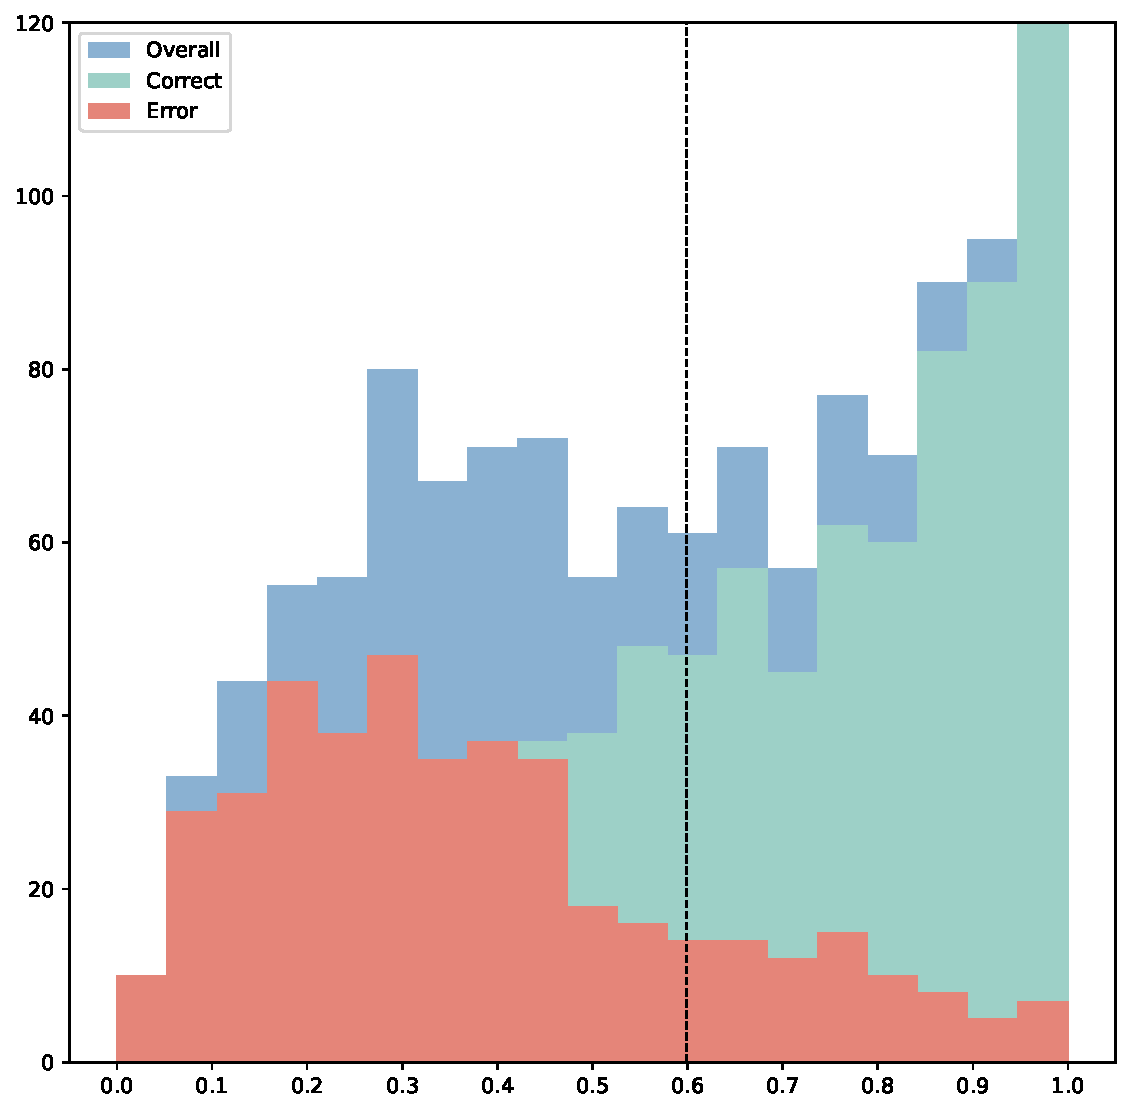
\includegraphics[width=\linewidth]{figs/supp_agreement_pc.pdf}\\[4pt]
{\small (b) Path-consistency}
\end{minipage}
\caption{Final answer agreement on GSM8K in the sentence-level experiments, with $C=0.8$ for PC. Blue shows all questions, green correct answers, and red incorrect answers. The panels use the same axis scales.}
\label{fig:sentence_agreement_final}
\end{figure}

\subsection{Illustrative reasoning trajectories}
Table~\ref{tab:sentence_example} illustrates progressive sentence-prefix reuse. Inherited text is retained while the newly generated suffix becomes shorter. It shows how the initial approach reused complete reasoning steps, complementing the token-fraction example of the current method in Table~\ref{tab:prefix_case}.

\begin{table}[!htbp]
\centering\small
\caption{A sentence-level prefix example. Black text is reused and blue text is newly generated.}
\label{tab:sentence_example}
\begin{tabularx}{\linewidth}{@{}lX@{}}
\toprule
Question & A robe takes 2 bolts of blue fiber and half that much white fiber. How many bolts in total does it take?\\
\midrule
No prefix & \textcolor{blue}{To make a robe, we need 2 bolts of blue fiber and half that much white fiber. We can write this as 2 + 1/2 * 2. Now 1/2 * 2 = 1, so the equation becomes 2 + 1 = 3. The answer is 3.}\\
\midrule
Level 1 & To make a robe, we need 2 bolts of blue fiber and half that much white fiber. \textcolor{blue}{2 * 1/2 = 1 bolt of white fiber. 2 + 1 = 3 bolts in total. The answer is 3.}\\
\midrule
Level 2 & To make a robe, we need 2 bolts of blue fiber and half that much white fiber. 2 * 1/2 = 1 bolt of white fiber. \textcolor{blue}{1 + 2 = 3 bolts in total. The answer is 3.}\\
\midrule
Level 3 & To make a robe, we need 2 bolts of blue fiber and half that much white fiber. 2 * 1/2 = 1 bolt of white fiber. 1 + 2 = 3 bolts in total. \textcolor{blue}{The answer is 3.}\\
\bottomrule
\end{tabularx}
\end{table}

A second example asks how much water remains after two girls each receive one sixth of 24 liters and a boy receives 6 liters. The correct answer is 10 liters. Table~\ref{tab:sentence_recovery} summarizes the Llama-3.2-1B-Instruct trajectories. Prefix levels increase and later return to zero; the final vote is correct despite earlier disagreement. The example shows that a return to unprefixed sampling can occur, but does not prove that the reused text was wrong or that recovery caused the correct final answer.

\begin{table}[!htbp]
\centering\small
\caption{Window-level summary of the water-allocation example. Tokens are the total newly generated tokens in each five-trajectory window. The recorded final answer is 10; answers 10 and 14 each receive seven votes.}
\label{tab:sentence_recovery}
\begin{tabular}{@{}rrlr@{}}
\toprule
Window & Prefix level & Sampled answers & Tokens\\
\midrule
1 & 0 & 8, 10, 14, 14, 14 & 383\\
2 & 1 & 2, 14, 14, 10, 16 & 283\\
3 & 2 & 10, 10, 10, 10, 12 & 89\\
4 & 0 & 16, 14, 2, 10, 14 & 380\\
\bottomrule
\end{tabular}
\end{table}

\subsection{Controller overhead and parallelism}
The sentence-level Llama-3-8B/GSM8K measurements in Table~\ref{tab:sentence_overhead} show that agreement evaluation and prefix selection take little time relative to model generation in that setting. They do not measure the full controller cost of the current method, which also ranks local confidence scores and manages trial and recovery.

\begin{table}[!htbp]
\centering\small
\caption{Controller timing in the supplementary 20-trajectory Llama-3-8B/GSM8K evaluation. Percentages are relative to the reported model-generation time.}
\label{tab:sentence_overhead}
\begin{tabular}{@{}lrr@{}}
\toprule
Component & Time (s) & Relative time (\%)\\
\midrule
Model generation & 2.2 & 100\\
Answer agreement evaluation & 0.000096 & 0.0044\\
Prefix construction & 0.00013 & 0.0059\\
\bottomrule
\end{tabular}
\end{table}

Windowed reuse also constrains parallelism. Trajectories within a window can run concurrently, but the next window depends on the preceding answers and prefix decision. Larger windows allow more concurrent generation, whereas smaller windows offer more frequent opportunities to extend a prefix. Token savings therefore need not translate into proportional latency reductions, especially when independent self-consistency trajectories can be served with greater parallelism.

\subsection{Prompt structure and scope}
The sentence-level experiments use few-shot demonstrations containing a question, reasoning, and final answer. Table~\ref{tab:sentence_prompts} summarizes their format without repeating the full demonstration sets. These prompts are distinct from the chat and thinking interfaces used in the main evaluation.
% Citation placeholders for the original CoT demonstrations and BIG-Bench Hard prompts.
% Full source demonstrations remain in paper/NIPS/appendix.tex.
\begin{table}[!htbp]
\centering\small
\caption{Prompt structure for the supplementary sentence-level experiments. Demonstrations supply intermediate reasoning followed by an explicit final answer.}
\label{tab:sentence_prompts}
\begin{tabularx}{\linewidth}{@{}lXX@{}}
\toprule
Task family & Demonstration content & Answer format\\
\midrule
Arithmetic reasoning & Arithmetic steps leading to a numerical result & The answer is [number].\\
StrategyQA & Short factual reasoning for a yes/no question & The answer is yes/no.\\
Ruin Names & Comparison of candidate humorous edits & The answer is [option].\\
Salient Translation & Comparison of a source sentence and its translation & The answer is [error-type option].\\
Boolean Expressions & Evaluation using logical operator precedence & The answer is True/False.\\
Tracking Shuffled Objects & State updates after successive swaps & The answer is [option].\\
Logical Deduction & Ordering objects from the supplied constraints & The answer is [option].\\
\bottomrule
\end{tabularx}
\end{table}

\paragraph{Implications for the current method.}
The initial experiments showed that reusing intermediate reasoning can shorten later trajectories across several short-chain tasks. They also exposed the trade-off between more aggressive reuse and accuracy preservation. The current method builds on this idea with one continuous shared prefix per window, a token-fraction length policy, local confidence selection, and explicit trial and recovery. The earlier results motivate this design direction; the experiments in Section~\ref{sec:evaluation} evaluate the resulting method.

These experiments do not train or modify the evaluated models. Their computational benefits and failure modes depend on the available reusable reasoning, the agreement threshold, and the generation interface. Reducing inference cost may improve accessibility but can also reduce the cost of harmful uses of the underlying models. Dataset text and model weights remain subject to their providers' terms and are not redistributed with the supplementary results.

\end{document}
